\documentclass[lettersize,journal]{IEEEtran}
\usepackage{amsmath,amsfonts}
\usepackage{algorithmic}
\usepackage{algorithm}
\usepackage{array}
\usepackage[caption=false,font=normalsize,labelfont=sf,textfont=sf]{subfig}
\usepackage{textcomp}
\usepackage{stfloats}
\usepackage{url}
\usepackage{verbatim}
\usepackage{graphicx}
\usepackage{cite}
\usepackage{amsthm}
\hyphenation{op-tical net-works semi-conduc-tor IEEE-Xplore}
% updated with editorial comments 8/9/2021

% Theorem-like environments with bold heads (e.g., Definition 1.)
\makeatletter
\@ifundefined{definition}{\newtheorem{definition}{Definition}}{}
\@ifundefined{example}{\newtheorem{example}{Example}}{}
\@ifundefined{problem}{\newtheorem{problem}{Problem}}{}
\makeatother

\begin{document}

\title{Distributed Task Allocation Under Temporal Logic and Communication Constraints with Resilient Task Coordination}

% \author{IEEE Publication Technology,~\IEEEmembership{Staff,~IEEE,}
%         % <-this % stops a space
% \thanks{This paper was produced by the IEEE Publication Technology Group. They are in Piscataway, NJ.}% <-this % stops a space
% \thanks{Manuscript received April 19, 2021; revised August 16, 2021.}}

% % The paper headers
% \markboth{Journal of \LaTeX\ Class Files,~Vol.~14, No.~8, August~2021}%
% {Shell \MakeLowercase{\textit{et al.}}: A Sample Article Using IEEEtran.cls for IEEE Journals}

% \IEEEpubid{0000--0000/00\$00.00~\copyright~2021 IEEE}
% Remember, if you use this you must call \IEEEpubidadjcol in the second
% column for its text to clear the IEEEpubid mark.

\maketitle

\begin{abstract}
This paper studies resilient distributed task allocation for heterogeneous multi-robot systems executing global syntactically co-safe linear temporal logic (sc-LTL) missions under range-limited communication. Such missions often arise in large-scale facilities, such as industrial plants and photovoltaic power stations, where robots with different capabilities must complete temporally ordered and collaborative subtasks across separated regions. However, large distances among target regions and sparse communication infrastructure may temporarily split the communication network into disconnected components, so robots cannot always obtain complete and timely team-state information. This lack of global execution awareness can block successor subtasks whose prerequisites cannot be confirmed, leave non-collaborative assignments unresolved when an assigned robot becomes unreachable or is removed, and invalidate collaborative subtasks when required robots are disconnected or removed. We first derive a temporally structured subtask representation from the global sc-LTL specification through NBA construction, pruning, and decomposition, and compute initial robot-level schedules through a consensus-based timetable algorithm (CBTA). The key contribution is a resilient execution layer that turns an initially feasible sc-LTL allocation into a recoverable distributed execution process when range-limited communication or robot removal makes the team-state information required by the allocation incomplete or stale. Rather than passively waiting for network-wide updates, robots move and gather to recover the information needed for execution, confirming prerequisite completion for dependent subtasks, returning individual tasks with unverifiable executors to distributed allocation, and re-forming collaborative teams with the required robot types and counts through coordinated reassignment. Simulations and physical multi-robot experiments demonstrate reliable mission completion and recovery under communication constraints and robot removal while satisfying temporal and collaborative requirements.
\end{abstract}

\begin{IEEEkeywords}
Linear Temporal Logic, Multi-robot Systems, Task Allocation, Multi-robot Coordination.
\end{IEEEkeywords}


\section{INTRODUCTION}
Multi-robot systems (MRS) are increasingly important in applications such as patrol, surveillance, and logistics \cite{qu2024novel,fang2025multi}, because robot teams can provide higher efficiency, robustness, and flexibility than a single robot can. Multi-robot task allocation (MRTA) is therefore a fundamental problem in MRS. Existing task-allocation methods are generally divided into centralized and distributed approaches. Centralized methods compute assignments through a coordinator with global information \cite{zhou2012task,okubo2022simultaneous}, but they often suffer from high computational cost and single-point-of-failure issues, which limit scalability and robustness in dynamic environments. By contrast, distributed methods allow robots to make decisions based on local information and limited communication, including auction-based algorithms \cite{wang2022consensus,govoni2025decentralized}, contract-net protocols \cite{wang2025multi}, and rule-based methods \cite{maoudj2016distributed}. These methods are especially attractive in communication-constrained scenarios such as security patrol and post-disaster search and rescue \cite{xie2017multi}.

However, many practical multi-robot missions are not only communication-constrained, but also subject to temporal requirements such as ordering, persistence, and synchronization \cite{leahy2016persistent}, which makes MRTA more challenging. To specify such requirements formally and precisely, recent studies have increasingly adopted formal languages \cite{11123780}, among which linear temporal logic (LTL) is one of the most widely used \cite{baier2008principles}. LTL provides a rigorous and unambiguous framework for task specification. For example, Li et al.\cite{li2025task} studied heterogeneous MRTA under global LTL specifications with variable robot capabilities and inter-task constraints. Yu et al.\cite{yu2021distributed} investigated fully distributed LTL-based multi-robot motion coordination using only local information, and employed online conflict detection and local replanning to preserve safety and specification feasibility. Despite this progress, sustaining global LTL missions in a distributed manner remains challenging under limited communication, because robots cannot maintain complete and timely team-state information during execution. Motivated by this challenge, this work develops a distributed task allocation framework with resilient task coordination under temporal logic and communication constraints.

Under LTL constraints, existing task allocation and planning methods can generally be classified into top-down and bottom-up approaches.
In top-down methods, a global LTL formula is used to specify the overall mission, and a centralized planner decomposes it into robot-level plans. A common strategy is to construct a product automaton from the nondeterministic Büchi automaton (NBA) derived from the global LTL formula and the discrete transition systems of the robots, and then solve the resulting graph-search problem \cite{smith2010optimal,ulusoy2013optimality}. However, this approach suffers from severe state explosion in multi-robot settings and is difficult to adapt to dynamic execution scenarios involving robot addition or removal.
Sampling-based methods~\cite{kantaros2018sampling,kantaros2020stylus} improve upon the above methods by constructing generation trees from NBA samples rather than from the full product automaton. However, such methods typically require the candidate robots for each subtask to be specified in advance. Luo et al.~\cite{luo2022temporal} formulated temporal-logic task allocation as a mixed-integer programming problem; however, it is difficult to adapt online to practical execution contingencies such as robot failures. Chen et al.~\cite{Chen2024RealTimeReactive} proposed an incremental decision-tree-based method that supports online adaptation, but it relies on global information. Recognizing the parallel and concurrent nature of MRS, some studies decompose a global specification into multiple subtasks using automaton transition relations to increase parallelism. Schillinger et al.~\cite{schillinger2018decomposition,schillinger2018simultaneous} decomposed the global task into a set of parallel subtasks. However, this method does not explicitly handle collaborative subtasks. Based on these works, Liu et al.~\cite{liu2024distributed,liu2024fast} further improved efficiency by representing subtask temporal relations with posets. Recent studies also combine large language models with optimization-based schedulers, such as DEXTER-LLM~\cite{zhu2025dexterllm}. Overall, although advanced top-down methods are effective at deriving task assignments from global temporal-logic specifications, can handle collaborative subtasks, and in some cases allow online adaptation, they still largely rely on centralized coordination and reliable global information. As a result, they are difficult to deploy with limited communication.

Bottom-up approaches, in contrast, usually assume that each robot is assigned a local temporal-logic task, and distributed coordination is then achieved through neighbor communication and online replanning. Filippidis et al.~\cite{6426027} proposed a distributed planning framework under temporal logic constraints that enables robots to exchange information and verify conflicts online. Each robot can communicate only with neighbors within its communication range, and a dedicated ``follower'' robot is used to establish and maintain communication links when interaction is required. In~\cite{guo2015multi,6907485}, each robot updates its knowledge based on local observations and propagates it through neighbor communication; with newly received knowledge, robots confirm and adjust their action paths online. However, such neighbor-only communication cannot guarantee that all robots required for a collaborative subtask can mutually communicate when needed. For scenarios with collaborative tasks, Tian et al.~\cite{tian2021decentralized} proposed a distributed cooperative computation framework that decomposes task constraints via an interaction-edge product automaton, enabling robots to synthesize local trajectories in parallel using only neighborhood interaction information.
Most existing work focuses on avoiding physical collisions while overlooking task conflicts. Chen et al. \cite{chen2024distributed} addressed task-level conflict resolution under communication constraints by predicting the goals of robots beyond communication range.

Compared with top-down approaches, these methods are generally more robust to communication constraints. However, many of them rely on a key assumption that local tasks are known or preassigned in advance. This assumption limits their applicability in scenarios where only a global mission is available. Moreover, when communication is restricted to local neighborhoods, information exchange alone may be insufficient to reliably support collaborative subtasks that require multiple robots. Therefore, existing methods still leave an important gap for scenarios in which robots must derive executable local behavior from a global specification and sustain task execution under limited communication range.


This gap becomes particularly significant in practical applications such as industrial inspection, photovoltaic power station patrol, and large-scale facility monitoring, where communication is restricted and mission requirements are more naturally specified as a global LTL formula rather than as preassigned local tasks. In such settings, the main challenge lies not only in obtaining a feasible initial task assignment, but also in sustaining task coordination during execution under limited communication range. Because robots cannot maintain a complete and timely view of the team state, a subtask that is feasible at the planning stage may later become unrealizable because of sudden robot failures or other unexpected events. In particular, two major challenges arise during mission execution. First, a robot may be unable to verify whether the temporal prerequisites of one of its pending subtasks have been satisfied, which leads to task blocking. Second, a collaborative subtask may fail to start because the required robots do not arrive in time.
Existing recovery strategies, including role reassignment, task reprioritization, and subtask reissuing~\cite{fua2005cobos,choudhury2022dynamic,kalempa2021multi}, can alleviate these issues to some extent, but they often operate from fragmented local views. Consequently, repeated failures due to the lack of global information or delayed information propagation may substantially increase the overall mission completion time.

Motivated by these challenges, this work develops a distributed task allocation framework with resilient task coordination under temporal logic and communication constraints. In particular, the proposed method explicitly addresses two issues that are not systematically handled in prior work: task blocking caused by unconfirmed temporal prerequisites and collaborative-subtask failures caused by incomplete team-state information.
To address task blocking caused by unconfirmed prerequisite completion, a patrol mechanism is introduced to actively gather and relay task-state information. To improve the resilience of task coordination, especially for collaborative subtasks, a resilient task coordination mechanism is developed by integrating leader-based coordination, timeout-triggered recruitment, and free-market-based reassignment. Here, the free market is a designated rendezvous region where robots synchronize state information and recover failed subtasks based on a more complete view of the team state. By explicitly incorporating these coordination and recovery mechanisms into execution, the proposed framework improves the robustness of global mission execution under limited communication. The main contributions of this work are summarized as follows:

\begin{itemize}
\item We propose a distributed task allocation framework that integrates task allocation and resilient task coordination under temporal logic and communication constraints, enabling robot teams to sustain task execution from a global specification using  local  information.

\item To address task blocking under limited communication, a patrol mechanism is proposed to actively gather information when prerequisite subtasks are overdue but completion is unconfirmed.

\item To strengthen resilient task coordination for collaborative subtasks, two complementary mechanisms are designed: a leader-based coordination with timeout-triggered recruitment to reduce subtask failures, and a free-market-based reassignment to mitigate significant delays when failures occur.

\item Theoretical analysis establishes completeness and task-completion guarantees under the assumptions of this paper.
\end{itemize}

Notations: Let $\mathbb{N}$ and $[N]$ denote the set of natural numbers and the index set $\{1,\ldots,N\}$, respectively. Given a set $\mathcal{A}$, let $|\mathcal{A}|$ and $2^{\mathcal{A}}$ denote the cardinality and power set of $\mathcal{A}$, respectively.

\section{PRELIMINARIES}
LTL formulas are constructed from atomic propositions $\mathcal{AP}$ using Boolean operators and temporal operators. Atomic propositions represent basic Boolean variables whose values are evaluated as either true or false. Details can be found in \cite{baier2008principles}. LTL formulas can be translated into NBA.

\begin{definition}[Nondeterministic Büchi Automaton]\label{def1}
A nondeterministic Büchi automaton (NBA) is a tuple $\mathcal{B}=(\mathcal{S},\mathcal{S}_0,\Sigma,\delta,\mathcal{F})$, where $\mathcal{S}$ is a finite set of states, $\mathcal{S}_0\subseteq \mathcal{S}$ is the set of initial states, $\Sigma=2^{\mathcal{AP}}$ is the input alphabet, $\delta:\mathcal{S}\times\Sigma\to 2^{\mathcal{S}}$ is the transition function, and $\mathcal{F}\subseteq \mathcal{S}$ is the set of accepting states.
\end{definition}

Given an infinite word $\omega = \sigma_0\sigma_1\sigma_2\dots$ with $\sigma_i \in \Sigma$, a run $\rho = s_0s_1s_2\dots$ of the NBA $\mathcal{B}$ over $\omega$ is an infinite state sequence such that $s_0 \in S_0$ and $s_{i+1} \in \delta(s_i,\sigma_i)$ for all $i \ge 0$. The run $\rho$ is accepting if it visits states in $F$ infinitely often.
Accepting runs can be represented in a prefix–suffix structure, where the prefix $w_{\text{pre}}$ runs from an initial state to an accepting state, and the suffix $w_{\text{suf}}$ forms a cycle containing at least one accepting state.

This paper focuses on a special class of LTL formulas called syntactically co-safe LTL (sc-LTL) \cite{belta2017formal}. sc-LTL formulas restrict temporal operators to $\bigcirc$ (next), $\cup$ (until), and $\Diamond$ (eventually), and must be written in a positive normal form.


\section{PROBLEM STATEMENT}

\subsection{Environment and Multi-Robot System}
In a discrete workspace $\mathcal{W} \subseteq \mathbb{R}^2$, let $\mathcal{L}=\{l_1,l_2,\dots,l_M\}$ be $M$ pairwise disjoint target regions, i.e., $l_i\cap l_j=\emptyset$ for all $i\neq j$, where $i,j\in[M]$. Let $\mathcal{U}$ denote uninteresting regions, such as forbidden areas, and assume $l_i\cap\mathcal{U}=\emptyset$.

Given workspace $\mathcal{W}$, we consider a heterogeneous robot team $\mathcal{R} = \{ r_1, r_2, \dots, r_N\}$, where $N$ is the number of robots. The robots have $n_t$ different types, where each robot belongs to exactly one type. Let $\mathcal{T}=[n_t]$ denote the type index set. For each $i\in\mathcal{T}$, let $\mathcal{R}_i\subseteq\mathcal{R}$ denote the set of robots of type $i$. Then $\mathcal{R}=\bigcup_{i=1}^{n_t}\mathcal{R}_i$ and $\mathcal{R}_i\cap\mathcal{R}_j=\emptyset$, $\forall i\neq j$. For any robot $r_m$, its velocity and position are denoted by $v_m$ and $x_m$, respectively.
Consider a time sequence $\{ \tau_n = n \Delta t \}_{n \in \mathbb{N}}$ with sampling interval $\Delta t$.
For convenience, for any quantity $y$, $y(\tau_n)$ denotes the value or state of $y$ at time $\tau_n$. In other words, the argument $\tau_n$ indicates the realization of the corresponding variable evaluated at $\tau_n$.

Assuming communication range $D \in \mathbb{R}^+$, robots can only communicate with neighbors within this range. The neighbor set of robot $r_m$ at time $\tau_n$ is defined as: $\mathcal{N}_m(\tau_n) = \left\{ r_n \;\middle|\; \|x_m(\tau_n) - x_n(\tau_n)\| \leq D \right\}$. The communication frequency is denoted by $f_{\mathrm{com}}$ in Hz.

\subsection{Problem Description} \label{problem}

To better describe the problem, we first introduce the atomic propositions.
Let $a_{i,w}^m$ represent the action required for task completion, indicating that $w$ robots of type $i$ must execute this action at region $l_m \in \mathcal{L}$, where $i \in \mathcal{T}$, $w \in \mathbb{N}$, and $w \leq |\mathcal{R}_i|$. The following atomic propositions are then introduced: i) the atomic proposition $p_m$ is true when any robot is located in region $l_m$, and false otherwise; ii) the atomic proposition $l_{i,w}^m$ is true iff action $a_{i,w}^m$ has been completed.

To facilitate task allocation under temporal logic constraints, a task model is introduced to explicitly capture the relationships among subtasks, actions, and workspace information. This abstraction provides a unified representation for subsequent task allocation.

\begin{definition}[Task Model]
The task model is defined as $TM = (\mathcal{Q}, \mathcal{A}, \mathcal{W}, \mathrm{LA}, \mathrm{LC},  \mathrm{LW})$, where $\mathcal{Q} := \{ q_i \} \cup \{ \varepsilon_q \}$ is the set of subtasks and $\varepsilon_q$ is the null subtask; $\mathcal{A} := \{ a_{i,w}^m \mid m \in [M],\ i \in [n_t],\ w \in [|\mathcal{R}_i|] \} \cup \{ \varepsilon_a \}$, where $\varepsilon_a$ is the empty action. For notational simplicity, an action in $\mathcal{A}$ can be written as $a_j$, where $j$ is the index. $\mathcal{W}$ is the workspace; $\mathrm{LA}: \mathcal{Q} \to 2^{\mathcal{A}}$ associates each subtask with a set of actions, i.e., $\mathrm{LA}(q_i) \subseteq \mathcal{A}$; $\mathrm{LC}: \mathcal{A} \to \mathbb{R}_{\ge 0}$ indicates the cost required to execute an action; and $\mathrm{LW}: \mathcal{A} \to \mathcal{W}$ specifies the target region for an action (excluding $\varepsilon_a$).
\end{definition}


Given workspace $\mathcal{W}$ and NBA $\mathcal{B}$ corresponding to the LTL-specified global task $\varphi$, the plan for robot $r_k$ is defined as a subtask-action-time sequence $\Pi_k = \Pi_{0,k}\Pi_{1,k}\cdots \Pi_{h_k,k}$, where each entry $\Pi_{i,k}$ is a subtask-action-time tuple associated with robot $r_k$, and $h_k$ denotes the length of the plan. More specifically, $\Pi_{i,k} = (q_i, a_i, t_{i,k})$, where $q_i \in \mathcal{Q}$, $a_i \in \mathrm{LA}(q_i)$, and $t_{i,k}$ denote the assigned subtask, the corresponding action, and the action start time of the $i$-th entry in the plan of robot $r_k$, respectively. In particular, the action of $\Pi_{0,k}$ is $\varepsilon_a$ and the subtask is $\varepsilon_q$. To  simplify notation, we use $\Pi_{i,k}(q)$ to denote the subtask component of $\Pi_{i,k}$ and $\Pi_{i,k}(a)$ to denote its action component in the remainder of this paper.


\begin{example} \label{example1}
Consider a heterogeneous robot group $\mathcal{R} = \{r_1, r_2, r_3, r_4\}$, including two type-1 (e.g., inspection) and two type-2 (e.g., maintenance and manipulation) robots, performing distributed tasks in a large-scale industrial park. The target regions are $\mathcal{L} = \{l_1, l_2, l_3, l_4\}$. The task requires two type-1 robots to go to $l_1$ for a joint inspection of an abnormal facility status, and one type-2 robot must travel to a local service station at $l_2$ to perform an on-site handling operation. In addition, one type-1 and one type-2 robot must go to $l_3$ for a coordinated repair task. During this coordinated-repair period, no robot may pass through region $l_4$, which represents a hazardous area. Let $p_4$ denote the atomic proposition that any robot enters region $l_4$. The task can be described by the following sc-LTL formula.
\begin{equation} \label{eq:example_task}
\varphi = \Diamond l_{1,2}^1 \land \Diamond l_{2,1}^2 \land \Diamond (l_{1,1}^3 \land l_{2,1}^3 \land \neg p_{4})
\end{equation}
 \end{example}
% \begin{figure}[thpb]
%       \centering
%       % \framebox{\parbox{3in}{}}
%       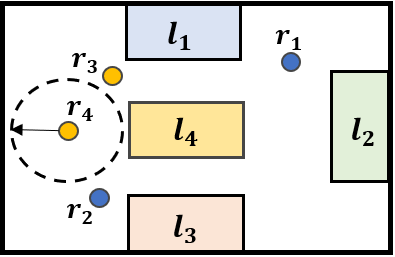
\includegraphics[scale=0.4]{image_4.png}
%       \caption{Schematic of the workspace. The blue circles denote type-1 robots, and the yellow circles denote type-2 robots.}
%       \label{workspace}
% \end{figure}

Based on the above, the problem studied in this work is described as follows.
\begin{problem}
Given a global sc-LTL task specification $\varphi$, workspace $\mathcal{W}$, and a team of heterogeneous robots $\mathcal{R}$, the goal is to develop a distributed task allocation and coordination strategy under limited communication range. Specifically, the strategy should generate a plan $\Pi_k$ for each robot $r_k \in \mathcal{R}$ and sustain task coordination during execution despite incomplete and delayed information. Let $\Pi := \{\Pi_k\}_{r_k \in \mathcal{R}}$ denote the collection of local plans. The objective is to generate $\Pi$ such that it satisfies $\varphi$. The following assumptions are made.

i) a robot can determine whether the task at a target region has been completed upon arrival;

ii) any robot within the broadcast range of a sender (another robot) will instantly receive its messages;

iii) the robot team contains sufficiently many robots of each required type.
\end{problem}


\section{FRAMEWORK OVERVIEW}


\begin{figure*}[t]
\centering
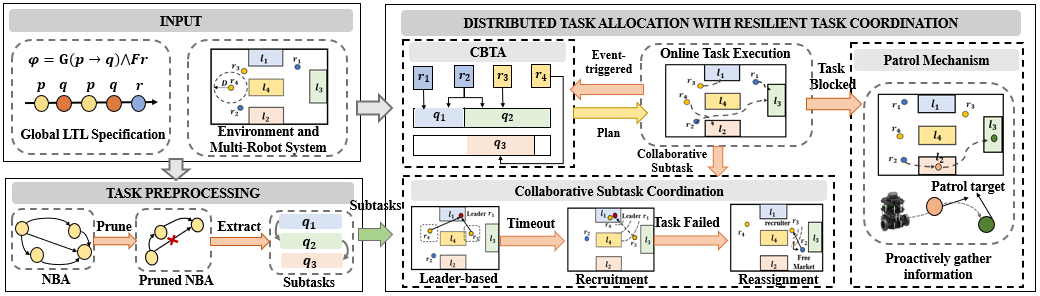
\includegraphics[width=\textwidth]{image_21.png}
\caption{Framework of the method. The framework consists of two stages: task preprocessing and distributed task allocation with resilient task coordination.}
\label{overall}
\end{figure*}

As shown in Fig.~\ref{overall}, the proposed framework consists of two parts: task preprocessing and distributed allocation with resilient task coordination.

In the task preprocessing part, the global sc-LTL specification is first translated into an NBA. The automaton is then pruned by removing infeasible and decomposable transitions, and the resulting pruned automaton is further decomposed into executable subtasks together with their temporal dependencies. 

In the second part, robots first generate initial plans through the consensus-based timetable algorithm (CBTA), which allocates optional subtasks. Since communication is limited, each robot maintains and broadcasts not only its own task state but also the peer information it has received. During execution, a robot may act as an ordinary executor, a temporary leader for a collaborative subtask, a recruiter in the free market, or a bidder responding to free-market recruitment. The proposed framework uses two execution mechanisms with different scopes: event-triggered replanning for ordinary local task execution, and free-market coordination for collaborative-failure recovery. Based on local information, robots maintain their local views of subtask progress and update their ordinary local plans through an event-triggered replanning mechanism. This mechanism is used only when a robot has a nonempty optional-subtask set and is not currently engaged in collaborative-recovery procedures. Here, collaborative-recovery procedures include timeout-triggered recruitment for collaborative subtasks and recruiter--bidder-based reassignment in the free market.

For collaborative subtasks, the first robot arriving at the target region acts as a temporary leader to coordinate team formation and synchronize task execution. If all required robots arrive within the collaboration waiting time, the leader broadcasts a start signal and the collaborative subtask proceeds as planned. Otherwise, timeout-triggered recruitment is activated. The leader first attempts local recovery by recruiting available and type-compatible robots that are reachable through direct or multi-hop communication. If local recovery is insufficient, a recruiter may be dispatched to the free market. If the required team still cannot be formed within the prescribed coordination horizon, the leader declares the collaborative subtask failed, and the failed subtask will be handled through free-market-based reassignment.

In addition, when a robot cannot confirm that the temporal prerequisites of its pending subtasks have been satisfied, a patrol mechanism is activated to actively gather the missing task-state information. 

Overall, the framework starts from a global temporal logic task, derives distributed executable subtasks, generates initial plans, and then sustains task progress online through event-triggered replanning, collaborative coordination, and patrol-based information gathering under limited communication.

\section{TASK PREPROCESSING}
To address Problem 1, we preprocess $\varphi$. As shown in Fig.~\ref{overall}, preprocessing has two phases: i) NBA pruning; and ii) task decomposition on the pruned NBA to obtain the subtask set $\mathcal{Q}$ and the temporal relations among subtasks.


\subsection{Pruning of NBA}
The LTL formula is first converted into an NBA $\mathcal{B}$ and then pruned to remove redundancies, yielding a simplified automaton $\mathcal{B}^-$. Specifically, there are two types of pruning:
\begin{itemize}
\item \emph{Removal of infeasible transitions:} removing transitions that cannot be realized, e.g., when the required number or types of robots exceed those available.
\item \emph{Elimination of decomposable transitions:} decomposable transitions are removed to improve task decomposition effectiveness~\cite{luo2024decomposition}.
\end{itemize}

A decomposable transition is defined as follows.

\begin{definition}[Decomposable Transition]\label{def:decomposable_transition}
In NBA $\mathcal{B}$, a transition from state $s_i$ to $s_j$ is called decomposable if there exists another state $s_k$ such that, for any $\sigma_{ik}, \sigma_{kj} \subseteq \Sigma$ satisfying $s_k \in \delta(s_i,\sigma_{ik})$ and $s_j \in \delta(s_k,\sigma_{kj})$, it holds that $s_j \in \delta(s_i,\sigma_{ik} \cup \sigma_{kj})$.
\end{definition}

% \begin{figure}[thpb]
%       \centering
%       % \framebox{\parbox{3in}{}}
%       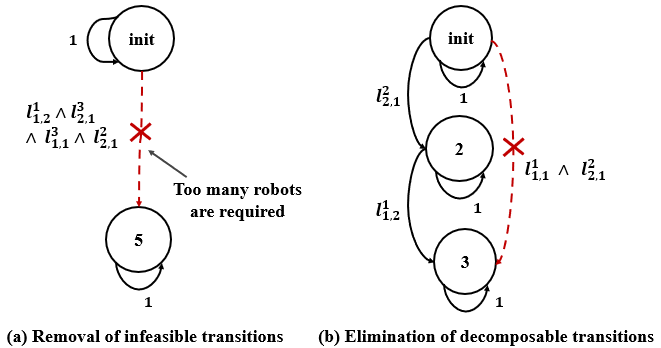
\includegraphics[scale=0.5]{image_9.png}
%       \caption{Pruning of the NBA automaton: (a) pruning infeasible transitions, illustrated by a case where the required number of robots is too large; (b) pruning decomposable transitions.}
%       \label{prune}
% \end{figure}

\textit{Lemma 1}\label{lem:pruning-preservation}: For any feasible word $w$ accepted by $\mathcal{B}$, there exists a corresponding word $w'$ accepted by $\mathcal{B}^{-}$.

\textit{Proof}: Consider an accepted word $w = \cdots \sigma_n \cdots$ with accepting run $\rho = \cdots s_i s_j \cdots$ in $\mathcal{B}$, where $s_j \in \delta(s_i,\sigma_n)$. The first pruning step removes only infeasible transitions, so every feasible accepted word is preserved. For the second pruning step, consider two cases.
For Case~1, if $\rho$ contains no decomposable transitions, then all transitions of $\rho$ remain in $\mathcal{B}^{-}$; hence $\rho$ is also an accepting run in $\mathcal{B}^{-}$ and we can set $w' = w$.
For Case~2, if a transition from $s_i$ to $s_j$ is removed as decomposable, there exists a state $s_k$ and labels $\sigma_{ik}, \sigma_{kj}$ such that $s_k \in \delta(s_i,\sigma_{ik})$, $s_j \in \delta(s_k,\sigma_{kj})$, and $\sigma_{ik} \cup \sigma_{kj} = \sigma_n$. Therefore, the transition $s_i \to s_j$ can be replaced by two transitions, $s_i \to s_k$ and $s_k \to s_j$. If both transitions $s_i \to s_k$ and $s_k \to s_j$ are non-decomposable, this reduces to Case~1. Otherwise, the same decomposition argument is applied recursively.
Because a transition cannot be decomposed indefinitely into realizable finite expressions, this recursive process terminates. The final constructed run has no decomposable transitions, so it reduces to Case~1 and is accepted by $\mathcal{B}^{-}$.

\subsection{Task Decomposition}
Following \cite{liu2024time}, $\mathcal{B}^-$ is decomposed into subtasks, and a relaxed partial order is extracted. A depth-first search on $\mathcal{B}^-$ generates an accepting path and its corresponding task sequence. Starting from this ordered sequence, subtasks are iteratively swapped, and each new path is checked for acceptability. This process relaxes unnecessary temporal constraints and yields a logically consistent subtask set that supports parallel execution, together with a relaxed partial order.

\begin{example}
  For the task in \textit{Example \ref{example1}}, the subtask set corresponding to $\varphi$ is given by $\Omega_{\varphi} = \left\{q_1, q_2, q_3\right\}$, where $q_1 = \{ 1, \{l^1_{1,2}\}, \{\}\}, q_2 = \{2, \{l^2_{2,1}\}, \{\}\}, q_3 = \{3,\{l^3_{1,1}, l^3_{2,1}\}, \{p_4\}\}$. Each subtask is represented by three entries: the first entry (e.g., 1, 2, 3) is the subtask index, the second set contains the actions to be executed, and the third set contains atomic propositions required on the self-loop.
\end{example}

\section{DISTRIBUTED ALLOCATION WITH RESILIENT TASK COORDINATION} \label{PLANNING}
This section describes how feasible plans are generated under limited communication,
and how these plans are executed under limited communication range.

\subsection{Consensus-based Timetable Algorithm} \label{CBTA}

To prevent robots from violating temporal logic constraints, the optional subtask set $\mathcal{O}_k(\tau_n)$ for robot $r_k$ is defined.
\begin{definition}[Optional Subtask Set]
At time $\tau_n$, the optional subtask set $\mathcal{O}_k(\tau_n)$ for robot $r_k$ includes all subtasks $q_i \in \mathcal{Q}$ that satisfy:
i) the numbers or types of robots committed to $q_i$ have not yet met the task requirements; ii) $r_k$ is unassigned and capable of $q_i$; iii) temporal constraints are satisfied.
\end{definition}

Note that robots committed to $q_i$ include those traveling to, waiting in, or executing the subtask at the target region. To reduce failures in collaborative subtasks, a robot commits only when its currently available information indicates that enough planned participants, in both number and required types, are already allocated to that subtask.

Allocation within $\mathcal{O}_k(\tau_n)$ is performed using CBTA \cite{wang2022consensus}, which can efficiently allocate tasks by iterative timetable construction and consensus-reaching among robots.
The cost of the current plan for robot $r_k$, i.e., the plan completion time, is defined below.
\begin{equation}\label{cost_k}
\mathrm{Cost}(\Pi_k(\tau_n)) = t_{h_k(\tau_n),k} - t_{0,k} + \mathrm{LC}(\Pi_{h_k(\tau_n),k}(a))
\end{equation}
Here, $h_k(\tau_n)$ is the current plan length of robot $r_k$ at time $\tau_n$; $t_{h_k(\tau_n),k}$ is the start time of the last action in $\Pi_k(\tau_n)$; $t_{0,k}$ is the start time of the plan; and $\mathrm{LC}(\Pi_{h_k(\tau_n),k}(a))$ is the execution cost of the last action.
   For each $q_i \in \mathcal{O}_k(\tau_n)$ and action $a_j \in \mathrm{LA}(q_i)$, candidate insertion positions after $\Pi_{0,k}(\tau_n)$ are evaluated by minimizing marginal cost, where $\Pi_{0,k}(\tau_n)$ is the initial tuple of the plan for robot $r_k$ at time $\tau_n$.
    The time component $t_{i,k} \in \Pi_{i,k}(\tau_n)$ is defined below.
\begin{equation}\label{start}
    t_{i,k} =
\begin{cases}
t_{0,k} + t_{\mathrm{left},k}+\dfrac{d_{i,k}}{v_k} , & \text{if } i = 1 \\
t_{i-1, k} + \mathrm{LC}(\Pi_{i-1,k}(a))+ \dfrac{d_{i-1,i}}{v_k} , & \text{otherwise}
\end{cases}
\end{equation}
where $t_{\mathrm{left},k}$ is the remaining time for the current subtask; for the case $i=1$, $d_{i,k}$ is the distance from $x_k(\tau_n)$ to the target region of $\Pi_{i,k}(q)$; and $d_{i-1,i}$ is the distance between the target regions of $\Pi_{i-1,k}(q)$ and $\Pi_{i,k}(q)$.
To enforce robot-quantity requirements, Eq.~(\ref{cost_k}) is augmented with a penalty $M \sum_{i \in [h_k(\tau_n)]}n_\mathrm{req}(\Pi_{i,k}(q))$, where $n_\mathrm{req}(\Pi_{i,k}(q))$ is the number of robots required to accomplish subtask $\Pi_{i,k}(q)$ and $M$ is a large constant.

Assume that $\mathcal{P}_k(\tau_n)$ is the set of plans received by robot $r_k$ at time $\tau_n$. Task-allocation conflicts are then resolved based on these shared plans as follows. For each candidate subtask $q_i \in \mathcal{O}_k(\tau_n)$ and each action $a_j \in \mathrm{LA}(q_i)$, robot $r_k$ first counts the number of robots currently assigned to execute $a_j$ according to $\mathcal{P}_k(\tau_n)$. Let $n_{\mathrm{req}}^k(a_j)$ denote the number of robots that $r_k$ estimates to be required for $a_j$. If the number of assigned robots exceeds $n_{\mathrm{req}}^k(a_j)$, an over-assignment conflict is detected. In this case, only the first $n_{\mathrm{req}}^k(a_j)$ robots with the earliest expected action start times are retained. Otherwise, no task-allocation conflict is identified, and all currently assigned robots are retained. See \cite{wang2022consensus} for algorithmic details. 

\begin{example}
For robot $r_1$ in \textit{Example 1}, suppose its optional subtask set is $\mathcal{O}_1(\tau_n) = \{q_1, q_3\}$ and the initial plan is $\Pi_1(\tau_n) = (\varepsilon_q, \varepsilon_a, \tau_n)$, where $\varepsilon_q$ and $\varepsilon_a$ denote empty subtask and action, respectively. The actions of robot $r_1$ for $q_1$ and $q_3$ are $a^1_{1,2}$ and $a^3_{1,1}$ with $\mathrm{LC}(a^1_{1,2})=2.6$ and $\mathrm{LC}(a^3_{1,1})=2.5$, where 2.6 and 2.5 denote the time required to complete the corresponding actions.   First, $a^1_{1,2}$ is inserted; at this stage it can only be placed after $\Pi_{0,1}$, yielding $\Pi_1(\tau_n)=(\varepsilon_q, \varepsilon_a, \tau_n)(q_1, a^1_{1,2}, \tau_n + 5.2)$. After that, $a^3_{1,1}$ is inserted; at this stage, it can be inserted either between $\Pi_{0,1}$ and $\Pi_{1,1}$ or after $\Pi_{1,1}$, and the corresponding marginal costs are 16.7 and 7.9, respectively. Then, $\Pi_1(\tau_n)$ is further updated to $(\varepsilon_q, \varepsilon_a, \tau_n)(q_1, a^1_{1,2}, \tau_n + 5.2)(q_3, a^3_{1,1}, \tau_n + 13.2)$.
\end{example}
% For robot $r_k$, if plan $\Pi_n(\tau_n)$ is nonempty and the time gap between $\tau_n$ and the current time $\tau_{\mathrm{now}}$ exceeds the information expiry time $T^{k,n}_{\mathrm{late}}$, it is excluded from planning. Excessive delays render information unreliable, and using outdated plans may cause deadlocks. $T^{k,n}_{\mathrm{late}}$ is determined by the robots’ communication status, $r_k$’s state at the last exchange and the robots’ positions, as defined in Eq.(\ref{late}).
% \begin{equation} \label{late}
%     T^{k,n}_{\mathrm{late}} =f_{\mathrm{com}}\left\lceil \left\lceil \frac{d_{k,n}}{D} \right\rceil \right\rceilT_{\mathrm{{enc}}}
% \end{equation}
% where $f_{\mathrm{com}} = \alpha_f + \beta_f(1 - N^k_{\mathrm{com}}/|\mathcal{R}|)$ is the communication density factor of robot $r_k$, with the tuning coefficients $\alpha_f$ and $\beta_f$. $N^k_{\mathrm{com}}$ is the number of robots that have communicated with robot $r_k$ during the past $T^k_{\mathrm{com}} = \alpha_c A_w / \left[(|\mathcal{R}| - 1)\pi D^2 v_k\right]$ seconds, where $\alpha_c$ is a coefficient, and $A_w$ is the area of workspace $\mathcal{W}$.
% $d_{k,n}$ denotes the distance between robot $r_k$'s current position and robot $r_n$'s estimated position. The estimation uses $r_n$'s last known location and task plan, assuming straight-line motion at a constant speed. The average encounter time $T_{\mathrm{enc}} = 1 / (4 D v_a \rho_r)$~\cite{bettstetter2004stochastic}, where $v_a$ is the average speed of robots and $\rho_r$ is the robot density.
%$d_{k,n}$ is the distance between the current position of $r_k$ and the estimated current position of $r_n$. The current position of $r_n$ is estimated based on its last known position $p_n$ at the time of the most recent communication, together with the subtask it was performing and its task plan. The estimation is carried out as follows: the current time is compared with the task start time in the plan to determine which task the robot is executing. If the current time exceeds the planned completion time of the task, the robot is considered to be in the free market (see \ref{info} for details). Otherwise, the robot is assumed to move at a constant speed along a straight line between task points, and its current position is estimated accordingly.
%is the distance to the target region last planned or approached by $r_n$ at their latest communication.


% \subsection{Event-Triggered Replanning Mechanism}
% %Due to limited communication, task conflicts may occur. Thus, a conflict detection and resolution mechanism is implemented.

% \subsubsection{Online Conflict Resolution}
% During plan execution, limited communication may lead to task conflicts. To address this issue, a conflict detection and resolution mechanism is introduced.

% To support this process, each robot classifies subtasks into three types at time $\tau_n$. i) Unassigned subtasks: subtasks for which the currently committed robots are still insufficient in number or type, so additional robots may still join. ii) Completed subtasks: subtasks whose required actions have already been executed and therefore no longer need allocation. iii) Confirmed subtasks: subtasks whose current commitments have been checked and verified to satisfy all participation requirements, meaning they are ready  for execution or being executed under the current  state . Let $\mathcal{T}^k_{\mathrm{not}}(\tau_n)$ and $\mathcal{T}^k_{\mathrm{already}}(\tau_n)$ denote the unassigned-subtask set and completed-subtask set maintained by robot $r_k$, respectively. During communication, robots exchange these sets and merge newly received updates. In this way, the optional subtask set is maintained online and remains consistent with the latest distributed task state.


% Each robot $r_k$ maintains and periodically broadcasts $\mathcal{S}_k(\tau_n)$, i.e., the robot-state information set collected by $r_k$ at time $\tau_n$. In particular, each robot broadcasts not only its own state but also the peer states it has received, enabling multi-hop information propagation. Formally,
% $\mathcal{S}_k(\tau_n)=\{\mathcal{S}_{m|k}(\tau_n)\mid r_m\in\mathcal{R},\ m\neq k\}$, and each element is defined as
% $\mathcal{S}_{m|k}(\tau_n)=\{\tau_m,q_m,a_m,t_a^m,t_s^m,{x}_{m}(\tau_n),\Pi_m(\tau_n)\}$, where each element records the latest status of robot $r_m$ as received by $r_k$ at time $\tau_n$. Specifically, $\tau_m$ is the generation timestamp of $r_m$'s latest status message; $q_m$ is the subtask currently committed by $r_m$; $a_m \in \mathrm{LA}(q_m)$ is the concrete action role that $r_m$ undertakes for $q_m$; $t_a^m$ is the estimated remaining travel time from $r_m$'s current estimated position to the target region of $q_m$; $t_s^m$ is the estimated task start time. Let $\mathcal{A}_m$ denote the set of estimated arrival times of other robots assigned to the same task region; then $t_s^m$ is defined as the difference of $r_m$'s own estimated arrival time and the $n_{\mathrm{req}}(a_m)$-th smallest element in $\mathcal{A}_m$ and is always non-negative. ${x}_{m}(\tau_n)$ denotes the position of $r_m$ at time $\tau_n$; and $\Pi_m(\tau_n)$ is the plan of robot $r_m$ at time $\tau_n$.

% Using the robot-state information set   $\mathcal{S}_k(\tau_n)$, the unassigned subtask set $\mathcal{T}^k_{\mathrm{not}}(\tau_n)$, and the completed subtask set $\mathcal{T}^k_{\mathrm{already}}(\tau_n)$, robot $r_k$ periodically checks for conflicts while executing $a_j \in \mathrm{LA}(q_i)$:
% i) Conflict caused by task completion:  At each check, $r_k$  verifies whether $q_i$ has entered $\mathcal{T}^k_{\mathrm{already}}(\tau_n)$. If yes, the current commitment is immediately invalidated because further motion for $q_i$ is redundant and may delay other pending tasks. Robot $r_k$ then stops and replans.
% ii) Over-assignment: If the number of robots committed to $a_j$ exceeds the required cardinality $n_{\mathrm{req}}(a_j)$, robot $r_k$ ranks all committed robots by their remaining travel time to the target region (smallest $t_a^m$ first) and keeps only the first $n_{\mathrm{req}}(a_j)$ robots as valid executors of $a_j$. If multiple robots have the same $t_a^m$, the tie is broken by robot ID in ascending order. If $r_k$ is not selected after this filtering step, it immediately stops the current commitment and replans.

% To support this mechanism, each robot classifies subtasks into three categories at time $\tau_n$: i) unassigned subtasks, whose currently committed robots are still insufficient in number or type, so additional robots may still join; ii) completed subtasks, whose required actions have already been executed and therefore no longer require allocation; and iii) confirmed subtasks, whose current commitments have been verified to satisfy all participation requirements and are thus ready for execution or are already under execution. Let $\mathcal{T}^k_{\mathrm{not}}(\tau_n)$ and $\mathcal{T}^k_{\mathrm{already}}(\tau_n)$ denote the unassigned-subtask set and completed-subtask set maintained by robot $r_k$, respectively. During communication, robots exchange these sets and merge newly received updates. In this way, the optional subtask set is maintained online and remains consistent with the latest distributed task state.

% Each robot $r_k$ maintains and periodically broadcasts a robot-state information set $\mathcal{S}_k(\tau_n)$, which records the information collected by $r_k$ at time $\tau_n$. In particular, each robot broadcasts not only its own state but also the peer states it has received, thereby enabling multi-hop information propagation. The robot-state information set is defined as $\mathcal{S}_k(\tau_n)=\{\mathcal{S}_{m|k}(\tau_n)\mid r_m\in\mathcal{R},\ m\neq k\}$. Each element $\mathcal{S}_{m|k}(\tau_n)$ is defined as follows: $\mathcal{S}_{m|k}(\tau_n)=\{\tau_m,q_m,a_m,t_a^m,t_s^m,{x}_{m}(\tau_n),\Pi_m(\tau_n)\}$.
% Here, $\mathcal{S}_{m|k}(\tau_n)$ records the latest status of robot $r_m$ as received by $r_k$ at time $\tau_n$. Specifically, $\tau_m$ is the generation timestamp of the latest status message from $r_m$; $q_m$ is the subtask currently committed by $r_m$; $a_m \in \mathrm{LA}(q_m)$ is the concrete action role undertaken by $r_m$ for $q_m$; $t_a^m$ is the estimated remaining travel time from the current estimated position of $r_m$ to the target region of $q_m$; and $t_s^m$ is the estimated task start time. Let $\mathcal{A}_m$ denote the set of estimated arrival times of other robots assigned to the same task region. Then $t_s^m$ is defined as the difference between the estimated arrival time of $r_m$ itself and the $n_{\mathrm{req}}(a_m)$-th smallest element in $\mathcal{A}_m$, and is always non-negative. In addition, ${x}_{m}(\tau_n)$ denotes the position of $r_m$ at time $\tau_n$, and $\Pi_m(\tau_n)$ denotes the plan of $r_m$ at time $\tau_n$.

% Based on the robot-state information set $\mathcal{S}_k(\tau_n)$, the unassigned-subtask set $\mathcal{T}^k_{\mathrm{not}}(\tau_n)$, and the completed-subtask set $\mathcal{T}^k_{\mathrm{already}}(\tau_n)$, robot $r_k$ periodically checks for conflicts while executing $a_j \in \mathrm{LA}(q_i)$. Two types of conflicts are considered.
% i) Conflict caused by task completion: At each check, $r_k$ verifies whether $q_i$ has entered $\mathcal{T}^k_{\mathrm{already}}(\tau_n)$. If so, the current commitment is immediately invalidated, since further motion for $q_i$ is redundant and may delay other pending tasks. Robot $r_k$ then stops and replans.
% ii) Over-assignment: If the number of robots committed to $a_j$ exceeds the required cardinality $n_{\mathrm{req}}(a_j)$, robot $r_k$ ranks all committed robots by their remaining travel time to the target region, with smaller $t_a^m$ taking higher priority, and keeps only the first $n_{\mathrm{req}}(a_j)$ robots as valid executors of $a_j$. If multiple robots have the same $t_a^m$, ties are broken by robot ID in ascending order. If $r_k$ is not selected after this filtering step, it immediately stops the current commitment and replans.

% \subsubsection{ Event-Triggered Replanning Mechanism}\label{None}

% Replanning is triggered by concrete state updates, including the reception of new state information from neighboring robots, task completion, detection of over-assignment conflicts, and failure events in  subtasks, which helps reduce unnecessary computation and avoids oscillations under limited communication.

% This mechanism is applied only to non-collaborative subtasks, because collaborative subtasks are handled by a dedicated resilient task coordination mechanism.
% For a non-collaborative subtask, the assigned robot may become unavailable during execution because of faults or other unexpected events and may therefore fail to complete the subtask. Under limited communication, other robots cannot directly distinguish such  failure. To adress this, each robot therefore uses a timeout-based rule to assess whether the subtask is failed and, if necessary, triggers local replanning.

% Specifically, if $\tau_{\mathrm{now}}-\tau_m > T_{\mathrm{late}}^k(q_m)$, robot $r_k$ treats the state record of $r_m$ as outdated and reassigns $q_m$ if $r_k$ can perform $a_m$, $q_m$ is non-collaborative, and $q_m \neq q_k$. Here, $\tau_m$ is the record timestamp, and $T_{\mathrm{late}}^k(q_m)$ is the expiry threshold adopted by robot $r_k$ for subtask $q_m$. This reassignment rule is restricted to non-collaborative subtasks because collaborative subtasks are handled by a separate coordination mechanism, which avoids mixing different recovery logics.

% Even for non-collaborative subtasks, delayed and incomplete information propagation may cause the same subtask to be assigned to multiple robots. Let $\mathcal{H}_k(q_m)=\{h\mid \mathcal{S}_{h|k}(\tau_n)\in \mathcal{S}_k(\tau_n),\ q_h=q_m\}$ denote the robot-index set induced by the state records in $\mathcal{S}_k(\tau_n)$, where $q_h$ is the subtask component in $\mathcal{S}_{h|k}(\tau_n)$. For each $h \in \mathcal{H}_k(q_m)$, robot $r_k$ computes a timeout candidate $T_{\mathrm{late}}^{k,h}$ by Eq.~(\ref{late-cand}) and uses the largest one as the expiry threshold for $q_m$. The expiry threshold is defined below.
% \begin{equation} \label{late}
%     T_{\mathrm{late}}^k(q_m) = \max_{h\in \mathcal{H}_k(q_m)} T_{\mathrm{late}}^{k,h}.
% \end{equation}

% The timeout candidate is defined below.
% \begin{equation} \label{late-cand}
% \begin{aligned}
% T_{\mathrm{late}}^{k,h} ={}& \alpha_{\mathrm{late}}\left(1 + \left\lceil \frac{d_{k,h}}{D} \right\rceil\right)
% \max\left(T_{\mathrm{enc}}, \frac{1}{f_{\mathrm{com}}}\right) \\
% & + t_s^h + \max_{a_i \in \mathrm{LA}(q_m)}\mathrm{LC}(a_i)
% \end{aligned}
% \end{equation}

% The average encounter time is defined below.
% \begin{equation} \label{enc}
% 	T_{\mathrm{enc}} = \frac{1}{4 D v_a \rho_r}
% \end{equation}
% where $\alpha_{\mathrm{late}}$ is a tuning parameter. In this paper, $\alpha_{\mathrm{late}}$ is set to 2.5 based on experimental results. The value is chosen to be greater than 1 so that the practical information expiration time remains above its theoretical estimate. $d_{k,h}$ denotes the distance between robot $r_k$'s current position and robot $r_h$'s estimated position. The position of $r_h$ is estimated based on its last known position $x_h$ at the most recent communication time, together with its task plan. The estimation is carried out as follows: the current time is compared with the subtask start time in the plan to determine which task the robot is executing. If the current time exceeds the planned completion time of that task, the robot is considered to be in the free market. Otherwise, the robot is assumed to move at a constant speed along a straight line between task points, and its current position is estimated accordingly. $T_{\mathrm{enc}}$ denotes the average encounter time~\cite{bettstetter2004stochastic}, where $v_a$ is the average speed of robots and $\rho_r$ is the robot density.

\subsection{Event-Triggered Replanning Mechanism}

The replanning mechanism described in this subsection is the CBTA-based update of local plans during online execution. It is used to revise ordinary local task assignments when newly received information changes a robot's view of the current task state. This mechanism is distinct from the free-market reassignment process for failed collaborative subtasks. In particular, CBTA replanning is used only when a robot has a nonempty optional-subtask set and is not currently engaged in collaborative-recovery procedures. Here, collaborative-recovery procedures include timeout-triggered recruitment for collaborative subtasks and recruiter--bidder-based reassignment in the free market. Therefore, ordinary replanning and collaborative-failure recovery are mutually exclusive at the robot level.



During execution, each robot $r_k$ maintains and periodically broadcasts a robot-state information set $\mathcal{S}_k(\tau_n)$, which records the information collected by $r_k$ at time $\tau_n$. In particular, each robot broadcasts peer states received from other robots, thereby enabling multi-hop information propagation. The robot-state information set is defined as $\mathcal{S}_k(\tau_n)=\{\mathcal{S}_{m|k}(\tau_n)\mid r_m\in\mathcal{R},\ m\neq k\}$. Each element $\mathcal{S}_{m|k}(\tau_n)$ is defined as follows: $\mathcal{S}_{m|k}(\tau_n)=\{\tau_m,q_m,a_m,t_a^m,t_s^m,{x}_{m}(\tau_n),\Pi_m(\tau_n)\}$.
Here, $\mathcal{S}_{m|k}(\tau_n)$ records the latest status of robot $r_m$ as received by $r_k$ at time $\tau_n$. Specifically, $\tau_m$ is the generation timestamp of the latest status message from $r_m$; $q_m$ is the subtask currently committed by $r_m$; $a_m \in \mathrm{LA}(q_m)$ is the concrete action role undertaken by $r_m$ for $q_m$; $t_a^m$ is the estimated remaining travel time from the current estimated position of $r_m$ to the target region of $q_m$; and $t_s^m$ is the estimated task start time. Let $\mathcal{A}_m$ denote the set of estimated arrival times of other robots assigned to the same task region. Then $t_s^m$ is defined as the non-negative difference between the estimated arrival time of $r_m$ itself and the $n_{\mathrm{req}}(a_m)$-th smallest element in $\mathcal{A}_m$. In addition, ${x}_{m}(\tau_n)$ denotes the position of $r_m$ at time $\tau_n$, and $\Pi_m(\tau_n)$ denotes the plan of $r_m$ at time $\tau_n$.

To reduce unnecessary computation under limited communication, CBTA replanning is triggered only by events that update a robot's local task view or indicate changes in task-execution status. Specifically, these events include the reception of task-state information with newer timestamps, completion or failure of the robot's current subtask, task-allocation conflicts, and failure inference for non-collaborative subtasks, as illustrated in Fig.\ref{event}.

\subsubsection{Conflict-Triggered Replanning}

During execution, limited communication may lead to task conflicts. To address this, a conflict-triggered replanning mechanism is introduced.

Each robot classifies subtasks into three categories at time $\tau_n$: i) unassigned subtasks, whose currently committed robots are still insufficient in number or type, so additional robots may still join; ii) completed subtasks, whose required actions have already been executed and therefore no longer require allocation; and iii) confirmed subtasks, whose current commitments have been verified to satisfy all participation requirements and are thus ready for execution or are already under execution. Let $\mathcal{T}^k_{\mathrm{not}}(\tau_n)$ and $\mathcal{T}^k_{\mathrm{already}}(\tau_n)$ denote the unassigned-subtask set and completed-subtask set maintained by robot $r_k$, respectively. During communication, robots exchange these sets and merge newly received updates. In this way, the optional subtask set is maintained online and remains consistent with the latest distributed task state.

Based on the robot-state information set $\mathcal{S}_k(\tau_n)$, the unassigned-subtask set $\mathcal{T}^k_{\mathrm{not}}(\tau_n)$, and the completed-subtask set $\mathcal{T}^k_{\mathrm{already}}(\tau_n)$, robot $r_k$ periodically checks for conflicts while executing $a_j \in \mathrm{LA}(q_i)$. Two types of conflicts are considered.
i) Conflict caused by task completion: At each check, $r_k$ verifies whether $q_i$ has entered $\mathcal{T}^k_{\mathrm{already}}(\tau_n)$. If so, the current commitment is immediately invalidated, since further motion for $q_i$ is redundant and may delay other pending tasks. Robot $r_k$ then stops and replans.
ii) Over-assignment: If the number of robots committed to $a_j$ exceeds the required cardinality $n_{\mathrm{req}}(a_j)$, robot $r_k$ ranks all committed robots by their remaining travel time to the target region, with smaller $t_a^m$ taking higher priority, and keeps only the first $n_{\mathrm{req}}(a_j)$ robots as valid executors of $a_j$. If multiple robots have the same $t_a^m$, ties are broken by robot ID in ascending order. If $r_k$ is not selected after this filtering step, it immediately stops the current commitment and replans.
\begin{figure}[thpb]
\centering
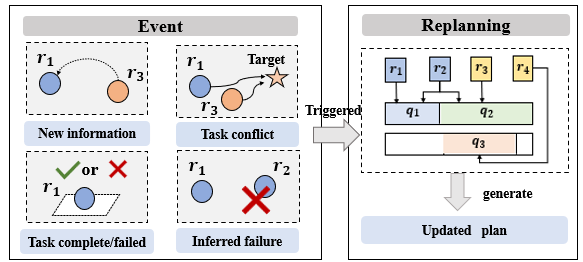
\includegraphics[scale=0.5]{image_22.png}
\caption{Schematic illustration of the event-triggered replanning mechanism}
\label{event}
\end{figure}

\subsubsection{Replanning for Non-Collaborative Subtasks} \label{None}




% The average encounter time is defined below.
% \begin{equation} \label{enc}
% 	T_{\mathrm{enc}} = \frac{1}{4 D v_a \rho_r}
% \end{equation}
% where $\alpha_{\mathrm{late}}$ is a tuning parameter. In this paper, $\alpha_{\mathrm{late}}$ is set to 2.5 based on experimental results. The value is chosen to be greater than 1 so that the practical information expiration time remains above its theoretical estimate. $d_{k,h}$ denotes the distance between robot $r_k$'s current position and robot $r_h$'s estimated position. The position of $r_h$ is estimated based on its last known position $x_h$ at the most recent communication time, together with its task plan. The estimation is carried out as follows: the current time is compared with the subtask start time in the plan to determine which task the robot is executing. If the current time exceeds the planned completion time of that task, the robot is considered to be in the free market. Otherwise, the robot is assumed to move at a constant speed along a straight line between task points, and its current position is estimated accordingly. $T_{\mathrm{enc}}$ denotes the average encounter time~\cite{bettstetter2004stochastic}, where $v_a$ is the average speed of robots and $\rho_r$ is the robot density.

This replanning is applied only to non-collaborative subtasks, because collaborative subtasks are handled by a dedicated resilient task coordination mechanism. For a non-collaborative subtask, the assigned robot may become unavailable during execution because of faults or other unexpected events and may therefore fail to complete the subtask. Under limited communication, other robots cannot directly distinguish such execution failure from delayed or incomplete information propagation. Therefore, each robot applies a timeout-based rule to assess whether the corresponding task-state record remains valid and, if necessary, triggers CBTA-based replanning when it has a nonempty optional-subtask set and is not currently engaged in collaborative-recovery procedures. In this way, non-collaborative timeout recovery remains in the ordinary replanning mechanism and is not merged into the free-market reassignment process.

Even for non-collaborative subtasks, delayed and incomplete information propagation may cause the same subtask to be assigned to multiple robots. Let $\mathcal{H}_k(q_m)=\{h\mid \mathcal{S}_{h|k}(\tau_n)\in \mathcal{S}_k(\tau_n),\ q_h=q_m\}$ denote the robot-index set induced by the state records in $\mathcal{S}_k(\tau_n)$, where $q_h$ is the subtask component in $\mathcal{S}_{h|k}(\tau_n)$. For each $h \in \mathcal{H}_k(q_m)$, robot $r_k$ computes a timeout candidate $T_{\mathrm{late}}^{k,h}$ by Eq.~(\ref{late-cand}) and uses the largest one as the expiry threshold for $q_m$. The expiry threshold is defined below.
\begin{equation} \label{late}
    T_{\mathrm{late}}^k(q_m) = \max_{h\in \mathcal{H}_k(q_m)} T_{\mathrm{late}}^{k,h}.
\end{equation}

The timeout candidate is defined below.
\begin{equation} \label{late-cand}
\begin{aligned}
T_{\mathrm{late}}^{k,h} ={}& \alpha_{\mathrm{late}}\left(1 + \left\lceil \frac{d_{k,h}}{D} \right\rceil\right)
\max\left(T_{\mathrm{enc}}, \frac{1}{f_{\mathrm{com}}}\right) \\
& + t_s^h + \max_{a_i \in \mathrm{LA}(q_m)}\mathrm{LC}(a_i)
\end{aligned}
\end{equation}

The average encounter time is defined below.
\begin{equation} \label{enc}
	T_{\mathrm{enc}} = \frac{1}{4 D v_a \rho_r}
\end{equation}
where $\alpha_{\mathrm{late}}$ is a tuning parameter. In this paper, $\alpha_{\mathrm{late}}$ is set to 2.5 based on experimental results. The value is chosen to be greater than 1 so that the practical information expiration time remains above its theoretical estimate. $d_{k,h}$ denotes the distance between robot $r_k$'s current position and robot $r_h$'s estimated position. The position of $r_h$ is estimated based on its last known position $x_h$ at the most recent communication time, together with its task plan. The estimation is carried out as follows: the current time is compared with the subtask start time in the plan to determine which task the robot is executing. If the current time exceeds the planned completion time of that task, the robot is considered to be in the free market. Otherwise, the robot is assumed to move at a constant speed along a straight line between task points, and its current position is estimated accordingly. $T_{\mathrm{enc}}$ denotes the average encounter time~\cite{bettstetter2004stochastic}, where $v_a$ is the average speed of robots and $\rho_r$ is the robot density.
Specifically, if current time $\tau_{\mathrm{now}}$ satisfies
$\tau_{\mathrm{now}}-\tau_m > T_{\mathrm{late}}^k(q_m)$, 
robot $r_k$ treats the state record of robot $r_m$ for subtask $q_m$ as outdated. If robot $r_k$ is capable of executing the corresponding action, $q_m$ is non-collaborative, $q_m \neq q_k$, and robot $r_k$ has a nonempty optional-subtask set while not being engaged in collaborative-recovery procedures, then robot $r_k$ triggers CBTA-based replanning, after which the updated local plan may take over $q_m$. Here, $\tau_m$ is the timestamp of the stored state record, and $T_{\mathrm{late}}^k(q_m)$ is the expiry threshold adopted by robot $r_k$ for subtask $q_m$.

Note that the event-triggered CBTA replanning mechanism is suspended whenever a robot is engaged in collaborative-recovery procedures. Once the robot is no longer engaged in timeout-triggered recruitment or free-market reassignment and again has a nonempty optional-subtask set, ordinary CBTA replanning can resume. In that case, failed collaborative subtasks are handled through the dedicated free-market reassignment mechanism rather than through CBTA-based local plan updates.

\subsection{Collaborative Subtask Coordination}
\subsubsection{Free Market}\label{info}
% The free market is a designated rendezvous place for two purposes: global information synchronization and failed-subtask reassignment. Robots enter this region in three cases: i) they currently have no executable pending subtask (unless all subtasks are already finished); ii) their assigned optional subtask cannot proceed because of failure or missing collaborators; and iii) they are explicitly dispatched by a leader as emergency recruiters.
% Robots broadcast the ID set of robots $\mathcal{R}_f$ currently in the free market and the corresponding timestamp, and then updates its locally maintained free-market ID set $\mathcal{R}_f$ according to the newest received timestamp.

% The free-market location is computed using entropy-based weighting of subtask information.
% For each subtask $q_i \in \mathcal{Q}$, two indicators are considered: the required robot count $N_i$ and the successor count $N_{\mathrm{suc},i}$. The normalized parameters $p_{i,1}$ and $p_{i,2}$ are computed as follows.
% \begin{equation}
% p_{i,1} = \frac{N_i}{\sum_{q_j \in \mathcal{Q}} N_j},
% \qquad
% p_{i,2} = \frac{N_{\mathrm{suc},i}}{\sum_{q_j \in \mathcal{Q}} N_{\mathrm{suc},j}}
% \end{equation}
% The entropy weights $w_k$ are computed as follows.
% \begin{equation}
% e_k = -\frac{1}{\ln |\mathcal{Q}|}
% \sum_{q_i \in \mathcal{Q}} p_{i,k} \ln p_{i,k},
% \qquad k \in \{1,2\}
% \end{equation}
% \begin{equation}
% w_k = \frac{1 - e_k}{\sum_{m=1}^{2} (1 - e_m)},
% \qquad k \in \{1,2\}
% \end{equation}
% where $e_k$ denotes the normalized entropy of indicator $k$, $k \in \{1,2\}$ (with $k=1$ for required robot count and $k=2$ for successor count), and $|\mathcal{Q}|$ is the number of subtasks. In the equation of $w_k$, $w_k$ is the entropy weight of indicator $k$, and $m$ is the indicator index used in the normalization denominator so that $\sum_{k=1}^{2} w_k = 1$.
% The entropy-weighted importance of subtask $q_i$ is computed as follows.

% \begin{equation}
% s_i = w_1 p_{i,1} + w_2 p_{i,2}
% \end{equation}

% \begin{equation}
% \bar{s}_i = \frac{s_i}{\sum_{q_j \in \mathcal{Q}} s_j}
% \end{equation}
% where $s_i$ is the unnormalized importance score of subtask $q_i$, and $\bar{s}_i$ is its normalized score. The normalization enforces $\sum_{q_i \in \mathcal{Q}} \bar{s}_i = 1$, so $\bar{s}_i$ can be used directly as a weight in center computation. Let $x_i$ denote the geometric center of subtask region $q_i$. The free-market center is computed as follows.
% \begin{equation}
% x_{\mathrm{free}} = \sum_{q_i \in \mathcal{Q}} \bar{s}_i x_i
% \end{equation}
% where $x_{\mathrm{free}}$ is the center of the free market. This equation is a weighted average of subtask-region centers; larger $\bar{s}_i$ makes subtask $q_i$ exert stronger influence on $x_{\mathrm{free}}$. If $x_{\mathrm{free}}$ lies in a forbidden region or outside the workspace, the final free-market location is set to the nearest feasible point.  In this work, a robot is considered to have arrived at the free market when it reaches a feasible point that is as close as possible to the free-market center and lies within the communication range of at least one robot already in the free market (if any).

The free market is a designated rendezvous region used for global information synchronization and failed-subtask reassignment. A robot enters this region in one of three situations: it has no executable pending subtask, unless all subtasks have already been completed; its assigned optional subtask cannot proceed because of failure or missing collaborators; or it is explicitly dispatched by a leader as an emergency recruiter. Robots broadcast the ID set of robots currently in the free market, denoted by $\mathcal{R}_f$, along with the corresponding timestamp. Upon receiving this information, each robot updates its locally maintained free-market ID set $\mathcal{R}_f$ using the newest timestamp.

The free-market location is computed by entropy-based weighting of subtask information. For each subtask $q_i \in \mathcal{Q}$, two indicators are considered: the required robot count $N_i$ and the number of successor subtasks $N_{\mathrm{suc},i}$. Their normalized forms are denoted by $\nu_{i,1}$ and $\nu_{i,2}$, respectively. They are defined below.
\begin{equation}
\nu_{i,1} = \frac{N_i}{\sum_{q_j \in \mathcal{Q}} N_j},
\qquad
\nu_{i,2} = \frac{N_{\mathrm{suc},i}}{\sum_{q_j \in \mathcal{Q}} N_{\mathrm{suc},j}}.
\end{equation}

The entropy weight of indicator $k$ is denoted by $w_k$, where $k=1$ corresponds to the normalized required robot count and $k=2$ corresponds to the normalized successor count. The normalized entropy $e_k$ is defined below.
\begin{equation}
e_k = -\frac{1}{\ln |\mathcal{Q}|}
\sum_{q_i \in \mathcal{Q}} \nu_{i,k} \ln \nu_{i,k},
\qquad k \in \{1,2\},
\end{equation}
The entropy weight $w_k$ is defined below.
\begin{equation}
w_k = \frac{1 - e_k}{\sum_{m=1}^{2} (1 - e_m)},
\qquad k \in \{1,2\}.
\end{equation}
Here, $|\mathcal{Q}|$ is the number of subtasks, and the denominator ensures that $\sum_{k=1}^{2} w_k = 1$.
The entropy-weighted importance of subtask $q_i$ is defined below.
\begin{equation}
s_i = w_1 \nu_{i,1} + w_2 \nu_{i,2},
\end{equation}
Its normalized score is defined below.
\begin{equation}
\bar{s}_i = \frac{s_i}{\sum_{q_j \in \mathcal{Q}} s_j}.
\end{equation}
Here, $s_i$ is the unnormalized importance score of subtask $q_i$, and $\bar{s}_i$ is its normalized score. This normalization ensures that $\sum_{q_i \in \mathcal{Q}} \bar{s}_i = 1$, so $\bar{s}_i$ can be directly used as a weight in computing the center. Let $x_i$ denote the geometric center of the region associated with subtask $q_i$. The center of the free market is defined below.
\begin{equation}
x_{\mathrm{free}} = \sum_{q_i \in \mathcal{Q}} \bar{s}_i x_i.
\end{equation}
This expression is a weighted average of subtask-region centers. A larger value of $\bar{s}_i$ means that subtask $q_i$ has a stronger influence on $x_{\mathrm{free}}$. If $x_{\mathrm{free}}$ lies in a forbidden region or outside the workspace, the final free-market location is set to the nearest feasible point. In this work, a robot is regarded as having arrived at the free market when it reaches a feasible point that is as close as possible to the free-market center and lies within the communication range of at least one robot already in the free market, if such a robot exists.
\subsubsection{Leader-based Collaborative Subtask Coordination}\label{coor}
For collaborative subtasks, robots adopt a leader-based coordination strategy. One robot serves as a temporary leader to collect arrival information, synchronize decisions, and issue recruitment actions. Compared with fully leaderless coordination, this design reduces negotiation overhead and decision inconsistency, thereby improving coordination efficiency and execution robustness.

% Robots first synchronize arrivals under leader coordination; if the required team cannot be formed within the collaboration waiting time, timeout-triggered recruitment is activated; if recruitment still fails, the subtask is regarded as failed, and failed subtasks are reassigned in the free market.

\begin{algorithm}[H]
\caption{Timeout-Triggered Recruitment}
\label{alg:leader_timeout}
\begin{algorithmic}[1]
\STATE \textbf{Input:} collaborative subtask $q_c$, arrived-robot set $\mathcal{R}_{\mathrm{arr}}$, leader state-information set $\mathcal{S}_l(\tau_n)$, free-market location $x_{\mathrm{free}}$, free-market robot set $\mathcal{R}_f$, reachable robot set $\mathcal{R}_b$
\IF{$|\mathcal{R}_{\mathrm{arr}}| < n_{\mathrm{req}}(q_c)$}
\STATE Construct $\mathcal{R}_{\mathrm{fit}}^{l}$ from robots in $\mathcal{R}_b$ that are available and type-compatible with the missing roles of $q_c$.
\IF{$|\mathcal{R}_{\mathrm{arr}} \cup \mathcal{R}_{\mathrm{fit}}^{l}| \geq n_{\mathrm{req}}(q_c)$}
\STATE Recruit the required robots from $\mathcal{R}_{\mathrm{fit}}^{l}$.
\STATE Update $T_{\mathrm{wait}}$ via Eq.~(\ref{col}).
\IF{waiting time $t < T_{\mathrm{wait}}$}
\STATE Leader $r_l$ broadcasts a start signal for subtask $q_c$.
\ELSE
\STATE Leader $r_l$ announces failure of subtask $q_c$.
\ENDIF
\ENDIF

\STATE Construct $\mathcal{R}_{\mathrm{fit}}^{f}$ from robots in $\mathcal{R}_f$ that are type-compatible with the remaining missing roles of $q_c$.

\IF{$|\mathcal{R}_{\mathrm{arr}} \cup \mathcal{R}_{\mathrm{fit}}^{l} \cup \mathcal{R}_{\mathrm{fit}}^{f}| < n_{\mathrm{req}}(q_c)$}
\STATE Leader $r_l$ announces failure of subtask $q_c$.
\ENDIF

\STATE Extract $\{x_p(\tau_n)\mid r_p \in \mathcal{R}_{\mathrm{arr}}\}$ from $\mathcal{S}_l(\tau_n)$.
\STATE $r_p \leftarrow \arg\min_{r_p \in \mathcal{R}_{\mathrm{arr}}} d(x_p(\tau_n), x_{\mathrm{free}})$
\STATE Recruit robots in $\mathcal{R}_{\mathrm{fit}}^{l}$ and dispatch $r_p$ to the free market.

\STATE Compute timeout $T_{\mathrm{leave}}^p$ via Eq.~(\ref{bid}).
\IF{all required recruited robots arrive before timeout}
\STATE Leader $r_l$ broadcasts a start signal for subtask $q_c$.
\ELSIF{waiting time $t \geq T_{\mathrm{leave}}^p$ or recruitment fails}
\STATE Leader $r_l$ announces failure of subtask $q_c$.
\ENDIF

\ENDIF
\end{algorithmic}
\end{algorithm}

Upon arriving at a subtask region, robot $r_k$ broadcasts an arrival signal $e_k = \{t_e^k, q_k, a_k\}$, where $t_e^k$ is the arrival timestamp at the task region, and $q_k$ and $a_k$ denote the current subtask and the action performed by $r_k$, respectively. The robot that arrives first at the task region is selected as leader $r_l$ to prevent conflicts caused by asynchronous arrivals. Let $q_c$ denote the collaborative subtask currently coordinated by leader $r_l$. If the number of robots that arrive within the collaboration waiting time $T_\mathrm{wait}$ satisfies the requirement of $q_c$, the leader broadcasts a start signal and the robots begin executing the collaborative subtask. Likewise, after timeout-triggered recruitment, execution starts only after the recruited robots have arrived and the participation requirement of $q_c$ is satisfied. Otherwise, once the waiting time exceeds $T_\mathrm{wait}$, timeout-triggered recruitment is initiated.


The collaboration waiting time $T_\mathrm{wait}$ is dynamically determined using leader $r_l$'s robot-state information set $\mathcal{S}_l(\tau_n)$. It is defined below in terms of the earliest arrival time $T_\mathrm{early}$ and the latest arrival time $T_\mathrm{late}$.
\begin{equation}\label{col}
T_\mathrm{wait} = \left(1 + \beta_w\frac{n_{\mathrm{req}}(q_c)}{n_{\mathrm{req}}^{\max}}\right)(T_\mathrm{late}-T_\mathrm{early})
\end{equation}
where $\beta_w$ is an adjustment coefficient. In this paper, $\beta_w$ is set to 1.25 based on experiments. Here, $n_{\mathrm{req}}(q_c)$ denotes the number of robots required for subtask $q_c$, and $n_{\mathrm{req}}^{\max}=\max_{q_j\in\mathcal{Q}} n_{\mathrm{req}}(q_j)$ denotes the maximum robot requirement across all subtasks. This design uses the arrival-time spread $(T_\mathrm{late}-T_\mathrm{early})$ as the baseline waiting window and scales it by $n_{\mathrm{req}}(q_c)/n_{\mathrm{req}}^{\max}$, so subtasks requiring more robots are given a proportionally longer waiting time to improve collaboration success while avoiding excessive delay for smaller teams. The rationale is that larger teams are harder to synchronize under limited communication: more robots imply greater arrival-time variability, so the probability that all required robots arrive within a short window is lower.

When leader $r_l$ observes that the collaboration waiting time has reached $T_{\mathrm{wait}}$ and the number of arrived robots is still below the required cardinality for $q_c$, timeout-triggered recruitment is activated. The procedure is summarized in Algorithm~\ref{alg:leader_timeout}. The leader first performs local recovery. It scans the reachable robot set $\mathcal{R}_b$, which consists of robots currently discoverable by $r_l$ through direct links or multi-hop relays, and extracts robots that are both available and type-compatible with the missing roles of $q_c$. Here, available robots are those that are not executing other subtasks, are not already committed to recruitment, and have not been recruited by other robots. This locally feasible set is denoted by $\mathcal{R}_{\mathrm{fit}}^{l}$. If the union of $\mathcal{R}_{\mathrm{arr}}$ and $\mathcal{R}_{\mathrm{fit}}^{l}$ is sufficient to satisfy the requirement of $q_c$, the leader recruits the required robots from $\mathcal{R}_{\mathrm{fit}}^{l}$. The recruitment message includes the subtask ID of $q_c$, the missing number and type requirements, and the publication timestamp $\tau_n$.

During recruitment, leader $r_l$ broadcasts recruitment messages and follows a first-come-first-served strategy among received bids. Bidder $r_b \in \mathcal{R}_{\mathrm{fit}}^{l}$ applies according to message publication time. Upon receiving a bid from robot $r_b \in \mathcal{R}_{\mathrm{fit}}^{l}$, leader $r_l$ sends a lock request $\mathrm{I}_{\mathrm{lock}}^l = \{q_c, \mathrm{ID}_b\}$ to $r_b$, where $\mathrm{ID}_b$ is the ID of $r_b$. The unlocked bidder $r_b$ replies with $\mathrm{I}_{\mathrm{agree}}^b = \{q_c, \mathrm{ID}_b\}$ and becomes locked. Leader $r_l$ then broadcasts $\mathrm{I}_{\mathrm{finish}}^l = \{q_c\}$, and the locked robots proceed to $q_c$. Here, recruitment is regarded as successful only when the required replacement robots have accepted the recruitment request and arrived at the target region within the corresponding waiting bound. Leader $r_l$ continues broadcasting recruitment messages until the required robots are obtained or the recruitment exceeds $T_\mathrm{bid}$. The collaboration waiting time $T_{\mathrm{wait}}$ is then updated according to the predicted arrival times of the recruited robots. If the updated waiting bound is still exceeded before team formation is completed, the leader declares the subtask failed. The bidding timeout $T_{\mathrm{bid}}$ is defined below.
\begin{equation}
T_{\mathrm{bid}} = |\mathcal{R}|\,\frac{1}{f_{\mathrm{com}}}\,N_{\mathrm{round}} + t_{\mathrm{comp}},
\end{equation}
where $|\mathcal{R}|$ is the total number of robots, $N_{\mathrm{round}}$ is the number of recruiter--bidder message rounds required by the recruitment process, and $t_{\mathrm{comp}}$ is the computation time. In this paper, $N_{\mathrm{round}}$ is set to 5 and $t_{\mathrm{comp}}$ is set to 2.0~s.

If local recovery is insufficient, the leader expands the search to the free market. It first constructs a backup candidate set $\mathcal{R}_{\mathrm{fit}}^{f}$ from robots in $\mathcal{R}_f$ whose capabilities match the remaining missing roles of $q_c$. If the union of the arrived robots $\mathcal{R}_{\mathrm{arr}}$, the locally reachable candidates $\mathcal{R}_{\mathrm{fit}}^{l}$, and the free-market candidates $\mathcal{R}_{\mathrm{fit}}^{f}$ is still insufficient, the subtask is immediately treated as failed. Otherwise, the leader selects a recruiter $r_p$ from the arrived robots according to
\begin{equation*}
    r_p = \arg\min_{r \in \mathcal{R}_{\mathrm{arr}}} d(x_r(\tau_n), x_{\mathrm{free}}),
\end{equation*}
where $x_r(\tau_n)$ is the position of robot $r$ recorded in $\mathcal{S}_l(\tau_n)$. The recruitment procedure executed by recruiter $r_p$ in the free market is the same as the one used by leader $r_l$. Leader $r_l$ declares subtask failure if recruitment is unsuccessful within $T^p_\mathrm{leave}$. The leave timeout is defined below.
\begin{equation} \label{bid}
	T^p_\mathrm{leave} = \left(1 + \zeta \frac{d_\mathrm{leave}}{d_{\max}}\right) \left( \frac{2d_{\mathrm{leave}}}{v_p} \right) + T_{\mathrm{bid}}
\end{equation}
where \(d_{\max}\) is the maximum inter-target-region distance, and \(\zeta\) is an adjustment coefficient. Based on experiments, $\zeta$ is set to 0.75 in this paper. $d_{\mathrm{leave}}$ denotes the distance from recruiter $r_p$ to the free market. By adapting $T^p_\mathrm{leave}$ to travel distance, the leader avoids declaring failure too early for distant recruiters and avoids excessive waiting for nearby recruiters. The first term in Eq.~(\ref{bid}) estimates the round-trip travel time between the subtask region and the free market, while $T_{\mathrm{bid}}$ reserves time for recruitment in the market.

If recruitment is still unsuccessful within $T^p_\mathrm{leave}$, subtask $q_c$ is declared failed, and the leader notifies all robots currently executing $q_c$. Failed subtasks are added to each robot's failed-subtask set and are temporarily skipped until robots enter the free market.

% Subtask failure is not declared immediately when the required robots fail to arrive on time in the proposed method. Under limited communication, suitable idle robots may still be available outside the leader's current communication range, and declaring failure too early may therefore discard feasible recovery opportunities.

\subsubsection{Failure Handling for Collaborative Subtasks}

Failed collaborative subtasks are handled through free-market-based reassignment. Notably, the communication network among robots in the free market is assumed to be connected. Once state information is synchronized there, failed collaborative subtasks are reallocated through a recruiter--bidder mechanism, enabling robots to recover from collaboration failures using updated information. This mechanism is reserved for collaborative-failure recovery and does not replace the ordinary replanning mechanism for non-collaborative subtasks.

When robot $r_k$ finds that its current optional-subtask set contains only failed subtasks, it enters the free market for reassignment. After arriving at the free market, ordinary CBTA replanning remains inactive while $r_k$ waits to become, or acts as, a recruiter or bidder. Robot $r_k$ first synchronizes recruitment messages and state information, and then checks whether it should participate in the reassignment process as a recruiter or a bidder. Let $\mathcal{F}_k$ denote the failed-subtask set maintained by $r_k$. Let $\mathcal{R}_{\mathrm{rec}}$ denote the current recruiter set in the free market, and let $\mathcal{R}^{<}_k \subseteq \mathcal{R}_{\mathrm{rec}}$ denote the recruiters that published earlier than $r_k$. Robot $r_k$ becomes a recruiter only if it has not received any valid recruitment message for a compatible subtask. In that case, it selects one failed subtask from $\mathcal{F}_k$ according to the shortfall-and-distance rule and publishes a recruitment message for that subtask.

% For each required robot type $j \in \mathcal{T}$, define
% \begin{equation}
% n_{\mathrm{rem}}^{k}(t,j)
% =
% n_{\mathrm{free}}(t,j)
% -
% \sum_{\hat r \in \mathcal{R}^{\mathrm{earlier}}_k}
% n_{\mathrm{req}}(q_{\hat r},j),
% \end{equation}
% where $n_{\mathrm{free}}(t,j)$ is the number of free-market robots of type $j$ at time $t$, $n_{\mathrm{req}}(q,j)$ is the required type-cardinality for subtask $q$, and $\mathcal{R}^{\mathrm{earlier}}_k \subseteq \mathcal{R}^{\mathrm{act}}_{\mathrm{rec}}$ is the set of recruiters that published earlier than $r_k$.

% For each subtask $q \in \mathcal{F}_k$, the shortfall is calculated as follows.
% \begin{equation}
% \Delta(q)
% =
% \sum_{j \in \mathcal{T}}
% \max\!\left(0,\;n_{\mathrm{req}}(q,j)-n_{\mathrm{rem}}^{k}(t,j)\right).
% \end{equation}
% Recruiter $r_k$ selects the subtask with the minimum shortfall.
% \begin{equation}
% q_k^\ast
% =
% \arg\min_{q \in \mathcal{F}_k}
% \Delta(q).
% \end{equation}
% If multiple candidates share the same minimum shortfall, $r_k$ chooses the nearest subtask region. After determining the subtask to be handled first, $r_k$ publishes recruitment message $\mathrm{I}_{\mathrm{bid}}^k=\{\tau_k, r_k, q_k^\ast, \eta_k\}$, where $\tau_k$ is the publishing time and $\eta_k$ is the type-cardinality requirement vector of the recruitment message.

% In the free market, any robot that is not acting as a recruiter is treated as a bidder. Bidder $r_c$ applies according to task priority and recruitment-message publishing time. Let $\mathcal{M}_c(\tau_n)$ be the set of active recruitment messages received by bidder $r_c$ at time $\tau_n$, and let
% \begin{equation}
% \mathcal{M}^{\mathrm{com}}_c(\tau_n)=\left\{\mathrm{I}_{\mathrm{bid}}^p \in \mathcal{M}_c(\tau_n)\;\middle|\;\text{$r_c$ is compatible with }q_p\right\}.
% \end{equation}
% For each message $\mathrm{I}_{\mathrm{bid}}^p$, define $\rho(q_p)$ as the priority rank of subtask $q_p$ (smaller value means higher priority). The bidder choice is
% \begin{equation}
% p_c^\ast
% =
% \arg\min_{p:\,\mathrm{I}_{\mathrm{bid}}^p \in \mathcal{M}^{\mathrm{com}}_c(\tau_n)}
% \bigl(\rho(q_p),\tau_p\bigr),
% \end{equation}
% where minimization is lexicographic: bidders first select the highest-priority subtask, and if priorities are equal, they select the earliest published recruitment message. In this paper, high-priority subtasks refer to emergency subtasks issued by leader-dispatched recruiters, whereas low-priority subtasks refer to regular subtasks that are failed or currently unassigned.

% During recruitment, if a recruiter $r_p$ receives a compatible recruitment message $\mathrm{I}_{\mathrm{bid}}^h$ that it can execute as a bidder, and the currently available free-market robots are insufficient to satisfy both recruitments simultaneously, $r_p$ compares $(\rho(q_h),\tau_h)$ with $(\rho(q_p),\tau_p)$. If $\rho(q_h)<\rho(q_p)$, or if $\rho(q_h)=\rho(q_p)$ and $\tau_h<\tau_p$, then $r_p$ relinquishes its recruiter role, cancels its own recruitment, and switches to bidder mode for $\mathrm{I}_{\mathrm{bid}}^h$.

% Recruiter $r_p$ follows a first-come-first-served strategy among received bids the same as Sec.~\ref{coor}. Upon receiving a bid from robot $r_c$, recruiter $r_p$ sends a lock request $\mathrm{I_{lock}^p} = \{q_p, \mathrm{ID}_c\}$ to $r_c$, where $q_p$ is the recruited subtask and $\mathrm{ID}_c$ is $r_c$'s ID. The uncommitted bidder $r_c$ replies with $\mathrm{I_{agree}^c} = \{q_p, \mathrm{ID}_c\}$ and becomes locked. After successful recruitment, $r_p$ broadcasts $\mathrm{I^p_{finish}} = \{q_p\}$, and the locked robots then proceed to $q_p$.
% Robots are unlocked if they receive no messages from $r_p$ within $T_{\mathrm{send}}$ seconds (presumed recruiter failure) or if higher-priority subtasks arrive. Here, $T_{\mathrm{send}}$ is set as
% \begin{equation}
% T_{\mathrm{send}}=\left(1+\left\lceil \frac{d_{c,p}}{D} \right\rceil\right)\frac{1}{f_{\mathrm{com}}},
% \end{equation}
% where $d_{c,p}$ is the distance from bidder $r_c$ to recruiter $r_p$, $D$ is the communication range, and $f_{\mathrm{com}}$ is the communication frequency. They then transmit $\mathrm{I_{unlock}^c} = \{q_p, \mathrm{ID}_c\}$ to prompt $r_p$ to remove them from the locked-robot list $\mathcal{L}_p$.

Let $n_{\mathrm{rem}}^{k}(t,j)$ represent the remaining number of type-$j$ robots that are available to recruiter $r_k$ at time $t$ after accounting for earlier recruitment requests.
For each failed subtask $q \in \mathcal{F}_k$, the shortfall is defined below.
$
\Delta(q)
=
\sum_{j \in \mathcal{T}}
\max\!\left(0,\;n_{\mathrm{req}}(q,j)-n_{\mathrm{rem}}^{k}(t,j)\right).
$
Recruiter $r_k$ then selects the failed subtask with the minimum shortfall. The selected subtask is defined below.
\begin{equation}
q_k^\ast
=
\arg\min_{q \in \mathcal{F}_k}
\Delta(q).
\end{equation}
If multiple candidates share the same minimum shortfall, $r_k$ selects the one whose target region is nearest. After determining the subtask to be handled first, $r_k$ publishes a recruitment message $\mathrm{I}_{\mathrm{bid}}^k=\{\tau_k, r_k, q_k^\ast, \eta_k\}$.
Here, $\tau_k$ is the publishing time, and $\eta_k$ is the type-cardinality requirement vector of the recruitment message.

After recruitment messages are published, any robot in the free market that is not acting as a recruiter is treated as a bidder. Bidder $r_c$ selects a recruitment message according to task priority and message publishing time. Let $\mathcal{M}_c(\tau_n)$ be the set of active recruitment messages received by bidder $r_c$ at time $\tau_n$. The compatible message set is defined as
$
\mathcal{M}^{\mathrm{com}}_c(\tau_n)
=\left\{\mathrm{I}_{\mathrm{bid}}^k \in \mathcal{M}_c(\tau_n)\;\middle|\;\text{$r_c$ is compatible with $q_k^\ast$}\right\}.
$
For each message $\mathrm{I}_{\mathrm{bid}}^k$, let $\rho(q_k^\ast)$ denote the priority rank of subtask $q_k^\ast$, where a smaller value means higher priority. The bidder-selected recruitment message is defined as
$
\mathrm{I}_c^\ast
=
\arg\min_{\mathrm{I}_{\mathrm{bid}}^k \in \mathcal{M}^{\mathrm{com}}_c(\tau_n)}
\bigl(\rho(q_k^\ast),\tau_k\bigr),
$
where minimization is lexicographic: bidders first select the highest-priority subtask, and among subtasks with the same priority, they choose the earliest published recruitment message. In this paper, high-priority subtasks refer to emergency subtasks issued by leader-dispatched recruiters, whereas low-priority subtasks refer to failed or currently unassigned subtasks handled through free-market reassignment.

During recruitment, recruiter $r_k$ may receive a compatible recruitment message $\mathrm{I}_{\mathrm{bid}}^h$ and become a potential bidder. If the currently available free-market robots are insufficient to satisfy both recruitments simultaneously, $r_k$ compares $(\rho(q_h^\ast),\tau_h)$ with $(\rho(q_k^\ast),\tau_k)$. If $\rho(q_h^\ast)<\rho(q_k^\ast)$, or if $\rho(q_h^\ast)=\rho(q_k^\ast)$ and $\tau_h<\tau_k$, then $r_k$ relinquishes its recruiter role, cancels its own recruitment, and switches to bidder mode for $\mathrm{I}_{\mathrm{bid}}^h$.

Recruiter $r_k$ follows the same first-come-first-served rule described in Sec.~\ref{coor}. Let $\mathcal{L}_k$ denote the bidder set currently locked by recruiter $r_k$. Upon receiving a bid from robot $r_c$, recruiter $r_k$ sends a lock request
$\mathrm{I}_{\mathrm{lock}}^k = \{q_k^\ast,\mathrm{ID}_c\}$
to $r_c$, where $q_k^\ast$ is the recruited subtask and $\mathrm{ID}_c$ is the ID of $r_c$. The uncommitted bidder $r_c$ replies with
$\mathrm{I}_{\mathrm{agree}}^c = \{q_k^\ast,\mathrm{ID}_c\}$
and becomes locked. Once recruitment is completed, $r_k$ broadcasts
$\mathrm{I}_{\mathrm{finish}}^k = \{q_k^\ast\}$,
and locked robots then proceed to execute $q_k^\ast$.

A bidder is unlocked if it receives no message from recruiter $r_k$ within $T_{\mathrm{send}}$ seconds, which indicates a presumed recruiter failure, or if a higher-priority subtask arrives. The unlocking timeout is defined below.
\begin{equation}
T_{\mathrm{send}}
=
\left(1+\left\lceil \frac{d_{c,k}}{D} \right\rceil\right)\frac{1}{f_{\mathrm{com}}},
\end{equation}
where $d_{c,k}$ is the distance from bidder $r_c$ to recruiter $r_k$, $D$ is the communication range, and $f_{\mathrm{com}}$ is the communication frequency. In such cases, bidder $r_c$ transmits
$\mathrm{I}_{\mathrm{unlock}}^c = \{q_k^\ast,\mathrm{ID}_c\}$
to prompt $r_k$ to remove it from the locked-robot list $\mathcal{L}_k$.

% \subsection{Task Failure Recovery} \label{Fail}

% Distributed approaches may encounter task failures under limited communication. In this subsection, task-failure recovery is divided into two parts: i) failure handling for non-collaborative subtasks, and ii) failure handling for collaborative subtasks.


% For non-collaborative subtasks, failure specifically means that the assigned robot becomes unavailable due to faults or other unexpected events and therefore cannot complete the subtask. To address this issue, each robot uses a timeout-based rule to assess peer status. For a non-collaborative subtask currently executed by robot $r_m$, if no completion message for that subtask is received  wluoithin a specified threshold, other robots infer that $r_m$ may have failed, which may render the subtask uncompletable.

% Specifically, if $\tau_{\mathrm{now}}-\tau_m > T_{\mathrm{late}}^k(q_m)$, robot $r_k$ treats the state record of $r_m$ as outdated and reassigns $q_m$ if $r_k$ can perform $a_m$, $q_m$ is non-collaborative, and $q_m \neq q_k$. Here, $\tau_m$ is the record timestamp, and $T_{\mathrm{late}}^k(q_m)$ is the expiry threshold adopted by robot $r_k$ for subtask $q_m$. This reassignment rule is restricted to non-collaborative subtasks because collaborative subtasks are handled by a separate coordination mechanism, which avoids mixing different recovery logics.

% Even for non-collaborative subtasks, delayed and incomplete information propagation may cause the same subtask to be assigned to multiple robots. Let $\mathcal{H}_k(q_m)=\{h\mid \mathcal{S}_{h|k}(\tau_n)\in \mathcal{S}_k(\tau_n),\ q_h=q_m\}$ denote the robot-index set induced by the state records in $\mathcal{S}_k(\tau_n)$, where $q_h$ is the subtask component in $\mathcal{S}_{h|k}(\tau_n)$. For each $h \in \mathcal{H}_k(q_m)$, robot $r_k$ computes a timeout candidate $T_{\mathrm{late}}^{k,h}$ by Eq.~(\ref{late-cand}) and uses the largest one as the expiry threshold for $q_m$. The expiry threshold is defined below.
% \begin{equation} \label{late}
%     T_{\mathrm{late}}^k(q_m) = \max_{h\in \mathcal{H}_k(q_m)} T_{\mathrm{late}}^{k,h}.
% \end{equation}

% The timeout candidate is defined below.
% \begin{equation} \label{late-cand}
% \begin{aligned}
% T_{\mathrm{late}}^{k,h} ={}& \alpha_{\mathrm{late}}\left(1 + \left\lceil \frac{d_{k,h}}{D} \right\rceil\right)
% \max\left(T_{\mathrm{enc}}, \frac{1}{f_{\mathrm{com}}}\right) \\
% & + t_s^h + \max_{a_i \in \mathrm{LA}(q_m)}\mathrm{LC}(a_i)
% \end{aligned}
% \end{equation}

% The average encounter time is defined below.
% \begin{equation} \label{enc}
% 	T_{\mathrm{enc}} = \frac{1}{4 D v_a \rho_r}
% \end{equation}
% where $\alpha_{\mathrm{late}}$ is a tuning parameter. In this paper, $\alpha_{\mathrm{late}}$ is set to 2.5 based on experimental results. The value is chosen to be greater than 1 so that the practical information expiration time remains above its theoretical estimate. $d_{k,h}$ denotes the distance between robot $r_k$'s current position and robot $r_h$'s estimated position. The position of $r_h$ is estimated based on its last known position $x_h$ at the most recent communication time, together with its task plan. The estimation is carried out as follows: the current time is compared with the subtask start time in the plan to determine which task the robot is executing. If the current time exceeds the planned completion time of that task, the robot is considered to be in the free market. Otherwise, the robot is assumed to move at a constant speed along a straight line between task points, and its current position is estimated accordingly. $T_{\mathrm{enc}}$ denotes the average encounter time~\cite{bettstetter2004stochastic}, where $v_a$ is the average speed of robots and $\rho_r$ is the robot density.
% \subsubsection{Failure Handling for Non-collaborative Subtasks} \label{None}
% \subsubsection{Failure Handling for Collaborative Subtasks}

% Failed collaborative subtasks are handled through free-market-based reassignment. Notably, the communication network among robots in the free market is assumed to be connected. Once a robot enters the free market, failed subtasks are reallocated through a recruiter--bidder mechanism after state information is synchronized, enabling robots to recover from collaboration failures using updated information.

% When robot $r_k$ finds that its current optional-subtask set contains only failed subtasks, it enters the free market for reassignment. After arriving at the free market, $r_k$ first synchronizes recruitment messages and state information, and then checks whether it can serve as a recruiter. Let $\mathcal{F}_k$ denote the failed-subtask set maintained by $r_k$. Let $\mathcal{R}_{\mathrm{rec}}$ denote the current recruiter set in the free market, and let $\mathcal{R}^{<}_k \subseteq \mathcal{R}_{\mathrm{rec}}$ denote the recruiters that published earlier than $r_k$. Robot $r_k$ becomes a recruiter only if it has not received any valid recruitment message for a compatible subtask. In that case, it selects one failed subtask from $\mathcal{F}_k$ according to the shortfall-and-distance rule and publishes a recruitment message for that subtask.

% % For each required robot type $j \in \mathcal{T}$, define
% % \begin{equation}
% % n_{\mathrm{rem}}^{k}(t,j)
% % =
% % n_{\mathrm{free}}(t,j)
% % -
% % \sum_{\hat r \in \mathcal{R}^{\mathrm{earlier}}_k}
% % n_{\mathrm{req}}(q_{\hat r},j),
% % \end{equation}
% % where $n_{\mathrm{free}}(t,j)$ is the number of free-market robots of type $j$ at time $t$, $n_{\mathrm{req}}(q,j)$ is the required type-cardinality for subtask $q$, and $\mathcal{R}^{\mathrm{earlier}}_k \subseteq \mathcal{R}^{\mathrm{act}}_{\mathrm{rec}}$ is the set of recruiters that published earlier than $r_k$.

% % For each subtask $q \in \mathcal{F}_k$, the shortfall is calculated as follows.
% % \begin{equation}
% % \Delta(q)
% % =
% % \sum_{j \in \mathcal{T}}
% % \max\!\left(0,\;n_{\mathrm{req}}(q,j)-n_{\mathrm{rem}}^{k}(t,j)\right).
% % \end{equation}
% % Recruiter $r_k$ selects the subtask with the minimum shortfall.
% % \begin{equation}
% % q_k^\ast
% % =
% % \arg\min_{q \in \mathcal{F}_k}
% % \Delta(q).
% % \end{equation}
% % If multiple candidates share the same minimum shortfall, $r_k$ chooses the nearest subtask region. After determining the subtask to be handled first, $r_k$ publishes recruitment message $\mathrm{I}_{\mathrm{bid}}^k=\{\tau_k, r_k, q_k^\ast, \eta_k\}$, where $\tau_k$ is the publishing time and $\eta_k$ is the type-cardinality requirement vector of the recruitment message.

% % In the free market, any robot that is not acting as a recruiter is treated as a bidder. Bidder $r_c$ applies according to task priority and recruitment-message publishing time. Let $\mathcal{M}_c(\tau_n)$ be the set of active recruitment messages received by bidder $r_c$ at time $\tau_n$, and let
% % \begin{equation}
% % \mathcal{M}^{\mathrm{com}}_c(\tau_n)=\left\{\mathrm{I}_{\mathrm{bid}}^p \in \mathcal{M}_c(\tau_n)\;\middle|\;\text{$r_c$ is compatible with }q_p\right\}.
% % \end{equation}
% % For each message $\mathrm{I}_{\mathrm{bid}}^p$, define $\rho(q_p)$ as the priority rank of subtask $q_p$ (smaller value means higher priority). The bidder choice is
% % \begin{equation}
% % p_c^\ast
% % =
% % \arg\min_{p:\,\mathrm{I}_{\mathrm{bid}}^p \in \mathcal{M}^{\mathrm{com}}_c(\tau_n)}
% % \bigl(\rho(q_p),\tau_p\bigr),
% % \end{equation}
% % where minimization is lexicographic: bidders first select the highest-priority subtask, and if priorities are equal, they select the earliest published recruitment message. In this paper, high-priority subtasks refer to emergency subtasks issued by leader-dispatched recruiters, whereas low-priority subtasks refer to regular subtasks that are failed or currently unassigned.

% % During recruitment, if a recruiter $r_p$ receives a compatible recruitment message $\mathrm{I}_{\mathrm{bid}}^h$ that it can execute as a bidder, and the currently available free-market robots are insufficient to satisfy both recruitments simultaneously, $r_p$ compares $(\rho(q_h),\tau_h)$ with $(\rho(q_p),\tau_p)$. If $\rho(q_h)<\rho(q_p)$, or if $\rho(q_h)=\rho(q_p)$ and $\tau_h<\tau_p$, then $r_p$ relinquishes its recruiter role, cancels its own recruitment, and switches to bidder mode for $\mathrm{I}_{\mathrm{bid}}^h$.

% % Recruiter $r_p$ follows a first-come-first-served strategy among received bids the same as Sec.~\ref{coor}. Upon receiving a bid from robot $r_c$, recruiter $r_p$ sends a lock request $\mathrm{I_{lock}^p} = \{q_p, \mathrm{ID}_c\}$ to $r_c$, where $q_p$ is the recruited subtask and $\mathrm{ID}_c$ is $r_c$'s ID. The uncommitted bidder $r_c$ replies with $\mathrm{I_{agree}^c} = \{q_p, \mathrm{ID}_c\}$ and becomes locked. After successful recruitment, $r_p$ broadcasts $\mathrm{I^p_{finish}} = \{q_p\}$, and the locked robots then proceed to $q_p$.
% % Robots are unlocked if they receive no messages from $r_p$ within $T_{\mathrm{send}}$ seconds (presumed recruiter failure) or if higher-priority subtasks arrive. Here, $T_{\mathrm{send}}$ is set as
% % \begin{equation}
% % T_{\mathrm{send}}=\left(1+\left\lceil \frac{d_{c,p}}{D} \right\rceil\right)\frac{1}{f_{\mathrm{com}}},
% % \end{equation}
% % where $d_{c,p}$ is the distance from bidder $r_c$ to recruiter $r_p$, $D$ is the communication range, and $f_{\mathrm{com}}$ is the communication frequency. They then transmit $\mathrm{I_{unlock}^c} = \{q_p, \mathrm{ID}_c\}$ to prompt $r_p$ to remove them from the locked-robot list $\mathcal{L}_p$.

% Let $n_{\mathrm{rem}}^{k}(t,j)$ represent the remaining number of type-$j$ robots that are still available to recruiter $r_k$ at time $t$ after accounting for earlier recruitment requests.
% For each failed subtask $q \in \mathcal{F}_k$, the shortfall is defined below.
% $
% \Delta(q)
% =
% \sum_{j \in \mathcal{T}}
% \max\!\left(0,\;n_{\mathrm{req}}(q,j)-n_{\mathrm{rem}}^{k}(t,j)\right).
% $
% Recruiter $r_k$ then selects the failed subtask with the minimum shortfall. The selected subtask is defined below.
% \begin{equation}
% q_k^\ast
% =
% \arg\min_{q \in \mathcal{F}_k}
% \Delta(q).
% \end{equation}
% If multiple candidates share the same minimum shortfall, $r_k$ selects the one whose target region is nearest. After determining the subtask to be handled first, $r_k$ publishes a recruitment message $\mathrm{I}_{\mathrm{bid}}^k=\{\tau_k, r_k, q_k^\ast, \eta_k\}$.
% Here, $\tau_k$ is the publishing time, and $\eta_k$ is the type-cardinality requirement vector of the recruitment message.

% After recruitment messages are published, any robot in the free market that is not acting as a recruiter is treated as a bidder. Bidder $r_c$ selects a recruitment message according to task priority and message publishing time. Let $\mathcal{M}_c(\tau_n)$ be the set of active recruitment messages received by bidder $r_c$ at time $\tau_n$. The compatible message set is defined below.
% \begin{equation}
% \mathcal{M}^{\mathrm{com}}_c(\tau_n)
% =\left\{\mathrm{I}_{\mathrm{bid}}^k \in \mathcal{M}_c(\tau_n)\;\middle|\;\text{$r_c$ is compatible with $q_k^\ast$}\right\}.
% \end{equation}
% For each message $\mathrm{I}_{\mathrm{bid}}^k$, let $\rho(q_k^\ast)$ denote the priority rank of subtask $q_k^\ast$, where a smaller value means higher priority. The bidder-selected recruitment message is defined below.
% \begin{equation}
% \mathrm{I}_c^\ast
% =
% \arg\min_{\mathrm{I}_{\mathrm{bid}}^k \in \mathcal{M}^{\mathrm{com}}_c(\tau_n)}
% \bigl(\rho(q_k^\ast),\tau_k\bigr),
% \end{equation}
% where minimization is lexicographic: bidders first select the highest-priority subtask, and among subtasks with the same priority, they choose the earliest published recruitment message. In this paper, high-priority subtasks refer to emergency subtasks issued by leader-dispatched recruiters, whereas low-priority subtasks refer to low-priority subtasks that are failed or currently unassigned.

% During recruitment, recruiter $r_k$ may itself receive a compatible recruitment message $\mathrm{I}_{\mathrm{bid}}^h$ and become a potential bidder. If the currently available free-market robots are insufficient to satisfy both recruitments simultaneously, $r_k$ compares $(\rho(q_h^\ast),\tau_h)$ with $(\rho(q_k^\ast),\tau_k)$. If $\rho(q_h^\ast)<\rho(q_k^\ast)$, or if $\rho(q_h^\ast)=\rho(q_k^\ast)$ and $\tau_h<\tau_k$, then $r_k$ relinquishes its recruiter role, cancels its own recruitment, and switches to bidder mode for $\mathrm{I}_{\mathrm{bid}}^h$.

% Recruiter $r_k$ follows the same first-come-first-served rule described in Sec.~\ref{coor}. Let $\mathcal{L}_k$ denote the bidder set currently locked by recruiter $r_k$. Upon receiving a bid from robot $r_c$, recruiter $r_k$ sends a lock request
% $\mathrm{I}_{\mathrm{lock}}^k = \{q_k^\ast,\mathrm{ID}_c\}$
% to $r_c$, where $q_k^\ast$ is the recruited subtask and $\mathrm{ID}_c$ is the ID of $r_c$. The uncommitted bidder $r_c$ replies with
% $\mathrm{I}_{\mathrm{agree}}^c = \{q_k^\ast,\mathrm{ID}_c\}$
% and becomes locked. Once recruitment is completed, $r_k$ broadcasts
% $\mathrm{I}_{\mathrm{finish}}^k = \{q_k^\ast\}$,
% and the locked robots then proceed to execute $q_k^\ast$.

% A bidder is unlocked if it receives no message from recruiter $r_k$ within $T_{\mathrm{send}}$ seconds, which indicates a presumed recruiter failure, or if a higher-priority subtask arrives. The unlocking timeout is defined below.
% \begin{equation}
% T_{\mathrm{send}}
% =
% \left(1+\left\lceil \frac{d_{c,k}}{D} \right\rceil\right)\frac{1}{f_{\mathrm{com}}},
% \end{equation}
% where $d_{c,k}$ is the distance from bidder $r_c$ to recruiter $r_k$, $D$ is the communication range, and $f_{\mathrm{com}}$ is the communication frequency. In such cases, bidder $r_c$ transmits
% $\mathrm{I}_{\mathrm{unlock}}^c = \{q_k^\ast,\mathrm{ID}_c\}$
% to prompt $r_k$ to remove it from the locked-robot list $\mathcal{L}_k$.


% % Robot \(r_m\) is considered available if  its current subtask $q_m$ is $\epsilon_q$ or
% % if \(t_{h_m(\tau_n),m} + \mathrm{LC}(a_{h_m(\tau_n)}) > \tau_{\mathrm{now}}\).
% % Robots with outdated information are defaulted to market presence.
% % \subsubsection{Free-market-based Reassignment}\label{outDeal}


% $r_l$ then broadcasts a failure message \(\mathrm{I_{fail}} \) to all robots executing \(q_l\). Upon receiving \(\mathrm{I_{fail}}\), \(r_n\) sends confirmation \(\mathrm{I_{sure}} \), adds \(q_l\) to its failed-subtask set \(\mathcal{F}_n\), and departs the task region. \(r_l\) terminates the subtask and adds \(q_l\) to \(\mathcal{F}_l\) after either:
% i) receiving \(\mathrm{I_{sure}}\) from all executing robots, or
% ii) waiting \(T_{\mathrm{out}}\) seconds after broadcasting \(\mathrm{I_{fail}}\).


\subsection{Patrol Mechanism for Task Blocking}

Temporal logic constraints can cause blocking while robots wait for prerequisite subtasks to be confirmed. For example, if subtask ``inspect Zone B'' is constrained to start only after ``verify tunnel entrance'' is completed, a robot assigned to Zone B may remain idle when the completion message from the entrance team cannot be received in time under limited communication. To address this issue, a patrol mechanism is proposed to proactively gather and relay prerequisite status information, thereby releasing blocked subtasks earlier.
Let \(\mathcal{Q}_k \subseteq \mathcal{Q}\) denote the set of subtasks executable by robot \(r_k\). For each \(q_i \in \mathcal{Q}_k\), let \(\mathcal{P}_i\) denote the prerequisite-subtask set of \(q_i\). For each prerequisite subtask \(q_j \in \mathcal{P}_i\), robot \(r_k\) maintains an estimated completion time \(\hat{t}_k(q_j)\). The estimate \(\hat{t}_k(q_j)\) is computed in the same form as \(T_{\mathrm{late}}^{k,m}\) in Sec.~\ref{None}. For subtasks constrained only by ``do not start before the prerequisite starts'', the same estimation logic is used, except that the prerequisite start time is estimated by subtracting the prerequisite execution duration from \(\hat{t}_k(q_j)\).

% , computed similarly to Eq.(\ref{col}) as follows.
% \begin{equation} \label{bid_cost3}
%      \hat{t}_k(q_j) = \tau_{\mathrm{s}} + \left(1 + \beta_o\frac{n_{\mathrm{req}}(q_j)}{n_{\mathrm{req}}^{\max}}\right)t_s^j + \max_{a_i \in \mathrm{LA}(q_j)}\mathrm{LC}(a_i)
% \end{equation}
% where \(\tau_{\mathrm{s}}\) is the timestamp, $\beta_o$ is an adjustment coefficient and \(t_s^j\) is the estimated start time. Note that if the constraint concerns subtask start time rather than completion time, the last term is omitted.

A robot triggers the patrol mechanism only when two conditions are simultaneously satisfied: i) there is no currently unassigned optional subtask that can be executed immediately, and ii) for at least one pending subtask \(q_i\), the current time exceeds the latest estimated completion time among its prerequisites, i.e., $\tau_{\mathrm{now}} > \max_{q_j \in \mathcal{P}_i} \hat{t}_k(q_j)$. This means the robot has waited beyond the expected prerequisite completion horizon but still cannot confirm prerequisite satisfaction from local information. In this case, the robot starts patrol to actively collect missing status updates. The initial patrol targets include all regions associated with unresolved prerequisite subtasks and the free market. During patrol, the target set is refined as follows: i) remove regions whose prerequisites are already completed or reliably verified, ii) skip prerequisites whose successor subtasks have already started, iii) omit prerequisites whose own predecessor conditions are still unmet, and iv) update optional-subtask candidates and their estimated completion times using newly gathered information. Once at least one executable optional subtask is identified, the robot exits patrol and switches to task execution.

After patrol, if the estimated completion time is updated, the robot will patrol again based on the new timing estimates; otherwise, it will wait \(t_p\) seconds before the next patrol. The patrol interval is defined below.
\begin{equation}
    t_{p} = \max_{q_i \in \mathcal{Q}_k}\max_{q_j \in \mathcal{P}_i} \left( \frac{d_f^j}{v_a} + \max_{a_\ell \in \mathrm{LA}(q_j)} \mathrm{LC}(a_\ell) \right)
\end{equation}
where \(d_f^j\) is the free-market-to-subtask distance. \(t_{p}\) assumes the subtask has failed and will be reassigned in the free market.

% \subssection{System Overview}

% As shown in Fig.~\ref{overall}, after preprocessing, robots plan optional subtasks via CBTA and execute them only when participant counts are met. During execution, $r_k$ detects conflicts via $\mathcal{S}_k(\tau_n)$ and $\mathcal{P}_k(\tau_n)$.
% To handle information inconsistencies, a free market is established based on task, environment, and robot properties.
% For collaborative subtasks, the earliest arriving robot  at the target region becomes leader $r_l$, who checks whether a recruiter should be dispatched to the free market to recruit additional robots.
%  Failed subtasks are reassigned via the free market and
% robots patrol to resolve task blocking caused by limited communication range.

\section{ALGORITHM ANALYSIS} \label{analysis}
%This section assesses the feasibility of the proposed algorithm, demonstrating deadlock avoidance and guaranteed task completion.
%\subsection{Feasibility}
This section proves that, under the assumptions in Sec.~\ref{problem} and a finite subtask set (i.e., $|\mathcal{Q}|<\infty$), the proposed algorithm guarantees task completion.

\textit{Theorem 1}: Failed collaborative subtasks handled through free-market reassignment are guaranteed to be completed.

\textit{Proof}: Consider a failed collaborative subtask $q$. For each type index $j \in \mathcal{T}$, let $n_{\mathrm{req}}(q,j)$ denote the required number of type-$j$ robots, and let $n_{\mathrm{free}}(t',j)$ denote the number of type-$j$ robots in the free market at time $t'$. Take any robot $r_k$ that is capable of executing $q$. We first show that $r_k$ enters the free market within a finite time $T_{\mathrm{bound}}^k$.
As long as the global task remains unfinished, a robot can stay in its current execution branch for only a finite waiting time before either completing the current subtask or switching to free-market recovery. This waiting time must cover both non-collaborative and collaborative cases. For non-collaborative subtasks, the waiting time is upper-bounded by the timeout threshold in Eq.~(\ref{late}); let the corresponding worst-case bound be denoted by $T_{\mathrm{nc}}^{\max}$. For collaborative subtasks, the waiting time is upper-bounded by the maximum collaboration waiting time in Eq.~(\ref{col}), together with the worst-case travel time to the free market, the recruitment time in the free market in Eq.~(\ref{bid}), and the worst-case return travel time. Let the corresponding worst-case bound be denoted by $T_{\mathrm{coll}}^{\max}$. Since each of these terms is finite under the assumptions of this paper, there exists a finite constant
\[
T_{\mathrm{wait}}^{\max}=\max\{T_{\mathrm{nc}}^{\max},\,T_{\mathrm{coll}}^{\max}\}
\]
such that no robot can remain indefinitely in an unfinished execution branch without either completing the current subtask or switching to free-market recovery.
For $q$, $r_k$ falls into one of three cases: i) $q \in \mathcal{F}_k$; ii) the currently available teammates are insufficient; iii) $q$ has been assigned to other robots but the collaboration cannot be completed successfully. In all three cases, if completion does not occur earlier, robot $r_k$ enters the free market after at most one such bounded waiting period for the current branch, together with at most one remaining subtask-execution interval. Let $T_{\mathrm{task}}^{\max,k}$ denote the maximum execution time of a subtask for robot $r_k$. The subtask execution time is finite, and co-safe LTL implies $|\mathcal{Q}|<\infty$. Therefore, robot $r_k$ enters the free market within a finite time satisfying
\begin{equation*}
T_{\mathrm{bound}}^k \le |\mathcal{Q}|\bigl(T_{\mathrm{task}}^{\max,k}+T_{\mathrm{wait}}^{\max}\bigr).
\end{equation*}

Now consider three cases for $q$. i) Recruitment proceeds without interruption by high-priority subtasks. Under assumption iii), together with the free-market coordination rule that higher-priority recruitments are resolved first and lower-priority requests are deferred rather than abandoned, robots capable of $q$ eventually become available within a finite time. Therefore, there exists a time $t' \in (t_0,\infty)$ such that
\begin{equation*}
\forall j \in \mathcal{T}, \quad n_{\mathrm{free}}(t',j) \ge n_{\mathrm{req}}(q,j).
\end{equation*}
Hence, $q$ can be successfully allocated. ii) The recruitment process is interrupted by emergency-subtask recruitment. Since $|\mathcal{Q}|<\infty$ and any departing robot $r_k$ is guaranteed to rejoin the free market within $T_{\mathrm{bound}}^k$, interruptions terminate in finite steps, which reduces to case i). iii) If $q$ remains unposted, it is because all capable robots are already engaged in earlier recruitments. Since every existing recruitment falls into case i) or ii), $q$ will eventually be posted. Hence, in all cases, $q$ will eventually be posted and successfully allocated.

\textit{Theorem 2}: Under assumptions ii) and iii), all subtasks are eventually completed.

\textit{Proof}: The feasibility of CBTA is discussed in \cite{wang2022consensus}. Under assumptions ii) and iii), an unfinished subtask can arise from one of the following situations: i) missing prerequisite-subtask information; ii) insufficient teammates for a collaborative subtask; or iii) failure of a robot assigned to a subtask during execution.
Case i) is resolved by the patrol mechanism. For case ii), insufficient teammates for a collaborative subtask eventually lead the relevant robots to the free market; by Theorem~1, the corresponding failed collaborative subtask is eventually reassigned and completed.
For case iii), first consider a non-collaborative subtask $q_m$ assigned to robot $r_m$. If $r_m$ does not complete $q_m$, then for any capable robot $r_k$, the stored record of $r_m$ is associated with the finite expiry threshold $T_{\mathrm{late}}^k(q_m)$ given by Eq.~(\ref{late}). Hence, after at most $T_{\mathrm{late}}^k(q_m)$ time beyond the timestamp of the latest stored record, some capable robot detects that the record of $r_m$ is outdated and, by the event-triggered replanning rule, triggers CBTA-based replanning to take over $q_m$. Therefore, non-collaborative execution failures are detected and recovered in finite time. If the failed subtask is collaborative, then the failure is handled through timeout-triggered recruitment and free-market reassignment, which again reduces to Theorem~1. Since $|\mathcal{Q}|<\infty$ and each unfinished subtask is recovered in finite time by one of the above mechanisms, all subtasks are eventually completed.

\textit{Theorem 3}: Under the assumptions of this paper, if the preprocessing stage yields a feasible decomposed task structure for $\varphi$, then the proposed execution framework preserves feasibility during online coordination and can complete the resulting subtasks through replanning, patrol, and free-market reassignment.

\textit{Proof}: By Lemma~1, automaton pruning preserves feasible words accepted by the original NBA. Therefore, if a feasible execution consistent with $\varphi$ exists, the preprocessing stage does not remove that feasibility at the automaton level. The subsequent task decomposition produces a subtask structure consistent with the temporal relations encoded in $\varphi$. During execution, non-collaborative disruptions are handled through event-triggered replanning, task blocking due to missing prerequisite information is handled by the patrol mechanism, and collaborative-subtask failures are handled through timeout-triggered recruitment and free-market reassignment. By Theorems~1 and~2, these recovery mechanisms ensure eventual completion of unfinished subtasks under the stated assumptions. Hence, feasibility is preserved through execution, and the decomposed task can be completed.

\section{RESULTS} \label{result}
%This section evaluates the proposed algorithm via simulations and physical experiments. LTL2BA \cite{10.1007/3-540-44585-4_6} is used to convert LTL formulas into NBA. The algorithm is implemented in Python 3 and tested on an 11th Gen Intel® Core™ i7-11390H with 16 GB RAM. Physical experiments run on Ubuntu 18.04 with ROS.
The algorithm is evaluated through simulations and physical experiments. LTL formulas are converted to NBAs using LTL2BA~\cite{10.1007/3-540-44585-4_6}. Simulations are run in Python 3 on an 11th Gen Intel® Core™ i7-11390H with 16~GB RAM. Physical experiments are conducted on Ubuntu 18.04 with ROS.

\subsection{Numerical Simulation}

We evaluate the proposed framework under communication-constrained settings, with a focus on its effectiveness in handling task blocking, dynamic robot changes, collaborative coordination, and failure recovery. To this end, the proposed framework is examined through four test scenarios:

i) Test 1 evaluates the patrol mechanism through an ablation study. For each instance, the patrol mechanism is enabled or disabled under the same task setting, while the communication range is varied to examine how efficiently blocked prerequisite subtasks are resolved and how this affects the final task completion rate.

ii) Test 2 compares timeout-triggered recruitment with timeout-based local recruitment~\cite{kalempa2021multi} under multiple communication ranges. This comparison is used to evaluate the impact of timeout-triggered recruitment on collaboration success and overall completion efficiency.

iii) Test 3 evaluates free-market-based reassignment in preventing repeated subtask failures, using failure-to-tail reassignment as a baseline with $D=1.5$\,m. The goal is to examine whether free-market-based reassignment can reduce repeated failure chains and improve recovery stability under limited communication.

iv) Test 4 evaluates the adaptability of the proposed framework to dynamic robot changes (e.g., robots joining or temporarily becoming unavailable during execution). We evaluate whether the framework can maintain feasible allocation updates and continue task progress without global replanning.
%The robot speed is set to 0.22 m/s according to its physical characteristics.

% The experimental  setup for Test 1 to Test 3 with 12 target regions $l = \{l_1, l_2, \dots, l_{12}\}$ and 12 robots of three types: type-1 (blue), type-2 (red), and type-3 (yellow). The  LTL-specified global task for Test 1 to Test 3 is:
% $\varphi = \Diamond(({l^{12}_{2,1}} \land {l^{12}_{1,1}})
% \land \Diamond( {l^7_{2,2}} \land \Diamond{l^6_{2,1}}))
% \land \Diamond{l^2_{3,1}}
% \land \Diamond{l^3_{3,1}}
% \land \Diamond{l^9_{3,3}}\land \lnot {p_4}$. After preprocessing $\varphi$, the resulting subtask set is $\Omega_{\varphi} = \left\{q_1, q_2, q_3, q_4, q_5, q_6\right\}$, where $q_1 = \{ 1, \{l^9_{3,3}\},\{p_4\}\}, q_2 = \{2, \{l^3_{3,1}\},\{p_4\}\}, q_3 = \{3,\{l^2_{3,1}\}, \{p_4\}\}, q_4 = \{4,\{l^{12}_{2,1}, l^{12}_{1,1}\},\{p_4\}\}, q_5 = \{5,\{l^7_{2,2}\},\{p_4\}\},q_6 = \{6,\{l^6_{2,1}\},\{p_4\}\}\}$.
The experimental setup consists of 12 target regions, denoted by $\mathcal{L} = \{l_1, l_2, \dots, l_{12}\}$, and a 12-robot team comprising three heterogeneous robot types: type-1, type-2, and type-3. The spatial arrangement of regions and robot deployment follows Fig.~\ref{workspace}. To evaluate robustness under different task-location assignments, we treat the region labels $l_1 \sim l_{12}$ as permutable and generate 25 randomized benchmark instances (Inst.~1--Inst.~25) by varying the label-to-location mapping while keeping the underlying workspace geometry unchanged.

\begin{figure}[thpb]
      \centering
        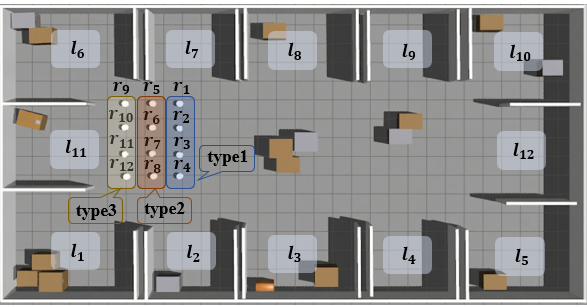
\includegraphics[scale=0.45]{image_23.png}
        \caption{
%
Simulation environment for Tests~1--4. The $30\times 15$ simulation environment contains 12 target regions $l_1 \sim l_{12}$ and 12 robots $r_1 \sim r_{12}$.
%30×15 environment contains 12 target regions ($l_1$ to $l_{12}$), 12 robots of 3 types (blue, red, yellow dots), and obstacles (black squares).
        	}
    \label{workspace}
   \end{figure}

\subsubsection{Test 1}
Consider the LTL-specified global task
$\varphi = \Diamond(({l^{12}_{2,1}} \land {l^{12}_{1,1}})\land \Diamond( ({l^7_{2,2}} \land \lnot ({l^{12}_{2,1}} \land {l^{12}_{1,1}})) \land  \Diamond({l^6_{2,1}}  \land \lnot l^7_{2,2})))\land \Diamond{l^2_{3,1}}\land \Diamond{l^3_{3,1}}\land \Diamond({l^9_{3,3}}\land \lnot {p_4})$. After preprocessing $\varphi$, the resulting subtask set is $\Omega_{\varphi} = \left\{q_1, q_2, q_3, q_4, q_5, q_6\right\}$, where $q_1 = \{1, \{l^9_{3,3}\},\{p_4\}\}$, $q_2 = \{2, \{l^3_{3,1}\},\{\}\}$, $q_3 = \{3,\{l^2_{3,1}\}, \{\}\}$, $q_4 = \{4,\{l^{12}_{2,1}, l^{12}_{1,1}\},\{\}\}$, $q_5 = \{5,\{l^7_{2,2}\},\{\}\}$,$q_6 = \{6,\{l^6_{2,1}\},\{\}\}$.
The objective of this experiment is to verify the causal role of the patrol mechanism in resolving task blocking under limited communication. To this end, we evaluate Inst.~1--Inst.~25 under two settings: Case~1 (with patrol) and Case~2 (without patrol), while keeping task instances, robot settings, and communication ranges identical. The only difference is whether robots are allowed to proactively gather information.

As shown in Fig.~\ref{diff_com}, when communication range decreases, Case 2 exhibits a significant decline in task completion rate because blocked robots cannot reliably obtain prerequisite updates and therefore remain in waiting states for long periods. Notably, Case 2 can still complete some instances at small communication ranges when a blocked robot happens to encounter another robot that already carries the required prerequisite information; however, this information-recovery path is opportunistic and unstable, and its success strongly depends on workspace geometry, robot trajectories, and task-region distribution. In contrast, Case 1 maintains a 100\% completion rate across all tested ranges: patrol converts passive waiting into active information acquisition, closes prerequisite-information gaps in a structured way, and enables blocked subtasks to be released in time without relying on chance encounters. These results highlight the key advantage of the patrol mechanism: it provides robust information recovery under communication constraints, rather than probabilistic recovery determined by incidental robot meetings.
% \begin{table}[h]

% 	\caption{TASK COMPLETION RATES UNDER DIFFERENT COMMUNICATION RANGES}
% 	\label{diff_com}
% 	\begin{center}
% 		\begin{tabular}{|c|c|c|c|c|c|}
% 			\hline
% 			$D$ (m) & 3.0 & 5.0 & 10.0 & 15.0 & 20.0 \\\hline
% 			Case 1 (with) & 100.0\% &  100.0\% & 100.0\% & 100.0\%  & 100.0\% \\\hline
% 			Case 2 (without) & 20\% & 52\% & 60\% & 96\%  & 100.0\%\\
% 			\hline
% 		\end{tabular}
% 	\end{center}
% \end{table}



\begin{figure}[thpb]
      \centering
        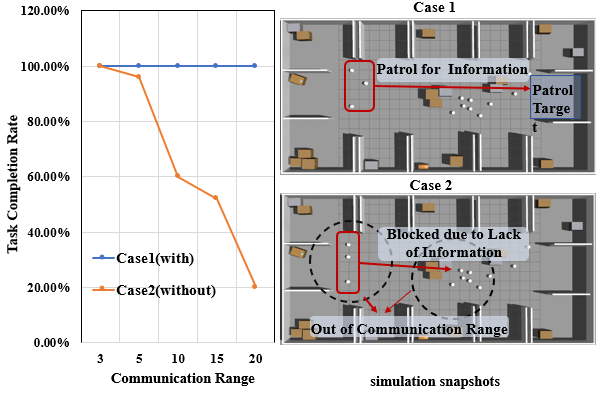
\includegraphics[scale=0.5]{image_24.png}
        \caption{
The results of Test 1. Left: task completion rates under different communication ranges. Right: simulation snapshots and an explanation of the differences between Case 1 (with patrol) and Case 2 (without patrol).}
\label{diff_com}
   \end{figure}
%To evaluate the effectiveness of the patrol mechanism, two cases are compared under Inst.1 to Inst.25: Case 1 with patrol mechanism and Case 2 without.  As shown in Tab. \ref{diff_com}, as the communication range decreases, the task completion rate drops significantly in the absence of the patrol mechanism because robots cannot receive updates on the completion of prerequisite subtasks. With the patrol mechanism, robots actively obtain information on the completion message of prerequisite subtasks; therefore, task blocking due to insufficient information is avoided, resulting in a 100\% task completion rate. Test 1 demonstrates that the patrol mechanism effectively resolves task blocking from missing information.
% time remains stable between 15 to 30~m despite decreasing communication range due to free-market robots relaying the completion message of $q_1$.  Below this range, robots rely on patrol for the message of $q_1$ updates (Fig. \ref{patrol}). Note that when $D$ is less than 15 m, disabling the patrol mechanism prevents robots from receiving  $q_1$'s completion message, leaving the task unfinished. Test 1 demonstrates that the patrol mechanism effectively resolves task blocking from missing information.

%With further range reduction, the free market can no longer relay messages, robots obtain information about $q_1$ completion through the patrol mechanism (Fig. \ref{patrol}). It should be noted that when , disabling the patrol mechanism prevents robots from receiving $q_1$'s completion message, resulting in the task remaining unfinished.
%Notably, at $D = 5$ m, disabling the patrolling mechanism prevents robots from receiving $q_1$’s completion message, causing the task to remain unfinished.

%\begin{figure}[thpb]
%	\centering
%	\includegraphics[scale=0.28]{pic/com15_trans.eps}
%	\caption{Completion message $q_1$ is transmitted along the red line. The black dashed line represents the boundary of the free market, and the brown dashed line depicts the movement trajectory of robots heading toward the free market.}
%%	{Task execution in Case 1 when $D=15$ m. The X-axis shows time, and the Y-axis lists subtasks. The wider block marks the robot’s current task; the narrower block in the subtask’s color means the robot is waiting for others. Gray lines indicate there is no assigned subtask and the robot is not in the free market.}
%	\label{com15}
%\end{figure}

%\begin{figure}[thpb]
%	\centering
%	\includegraphics[scale=0.42]{pic/patrol_time.eps}
%	\caption{Task timelines in Test 1 ($D=10$ m). The X-axis is time (seconds), the Y-axis is robots. Wide blocks denote subtasks, narrow colored blocks indicate waiting, and gray lines mean no subtask and not in the free market.}
%	\label{patrol}
%\end{figure}
\subsubsection{Test 2}

Considering the same global task $\varphi$ as in Test~1, we further evaluate timeout-triggered recruitment. Timeout-triggered recruitment (TTR) is compared with timeout-based local recruitment (TLR) \cite{kalempa2021multi}. The two methods differ only in how replacement candidates are searched after timeout: TLR selects from robots currently reachable by the leader (usually the nearest one), while TTR can dispatch a recruiter to the free market to obtain additional qualified robots outside the local communication neighborhood. In each run, one robot is randomly removed during execution of $q_1$ to create the same failure trigger for both methods.
Performance is measured by the completion time of type-3-related subtasks (T3-subtask time) under different communication ranges. We use this metric instead of total mission time because it directly captures recovery efficiency for the affected collaborative chain, while total mission time can be perturbed by unrelated subtasks.

Fig.~\ref{test2} and Table~\ref{tab:ttr_tlr_gap} show that TTR yields shorter T3-subtask time in most instances, with the largest gains at small communication ranges. The reason is that, under sparse connectivity, TLR is constrained by local visibility and may not find a feasible replacement quickly, whereas TTR expands the search scope through the free market and therefore restores collaboration earlier. When communication range is large, the free market is effectively inside the connected neighborhood, so TTR and TLR have similar candidate sets and similar performance. The exceptions (e.g., Inst.~2 and Inst.~6) are also explainable: both methods behave similarly because $q_2$ and $q_3$ are far from the initial robot positions and no suitable type-3 robot is available in the free market at timeout; here the dominant bottleneck is temporary resource scarcity, not the recruitment strategy. Overall, the experiment indicates that TTR improves robustness mainly by enlarging the effective replacement-search region under communication constraints.

\begin{table*}[!t]
\caption{T3-subtask time gap between TTR and TLR under different communication ranges. All time gaps are in seconds (s).}
\label{tab:ttr_tlr_gap}
\centering
\footnotesize
\setlength{\tabcolsep}{3.5pt}
\renewcommand{\arraystretch}{1.10}
{\setlength{\arrayrulewidth}{1.0pt}

\begin{tabular}{lccccccccccccc}
\hline
\textbf{D (m)} & \textbf{Inst. 1} & \textbf{Inst. 2} & \textbf{Inst. 3} & \textbf{Inst. 4} & \textbf{Inst. 5} & \textbf{Inst. 6} & \textbf{Inst. 7} & \textbf{Inst. 8} & \textbf{Inst. 9} & \textbf{Inst. 10} & \textbf{Inst. 11} & \textbf{Inst. 12} & \textbf{Inst. 13} \\\hline
3  & 11.29 & 0.03 & 19.56 & 27.82 & 16.75 & 0.12 & 16.22 & 52.07 & 21.69 & 21.69 & 0.32 & 17.09 & 36.36 \\
5  & 16.26 & 0.12 & 27.73 & 37.31 & 24.61 & 0.23 & 15.48 & 10.20 & 15.49 & 15.49 & 0.12 & 0.32 & 0.32 \\
10 & 26.13 & 0.02 & 0.00 & 43.70 & 0.11 & 0.09 & 0.00 & 10.28 & 27.52 & 27.52 & 0.22 & -0.25 & 0.32 \\\hline
\end{tabular}

\vspace{2pt}
\textit{Table~\ref{tab:ttr_tlr_gap} (continued)}
\vspace{2pt}

\begin{tabular}{lcccccccccccc}
\hline
\textbf{D (m)} & \textbf{Inst. 14} & \textbf{Inst. 15} & \textbf{Inst. 16} & \textbf{Inst. 17} & \textbf{Inst. 18} & \textbf{Inst. 19} & \textbf{Inst. 20} & \textbf{Inst. 21} & \textbf{Inst. 22} & \textbf{Inst. 23} & \textbf{Inst. 24} & \textbf{Inst. 25} \\\hline
3  & 20.43 & -0.19 & 23.10 & 18.41 & 13.53 & 0.32 & 19.91 & 26.17 & 0.27 & 16.93 & 22.85 & 0.12 \\
5  & 16.57 & -0.28 & 17.49 & 28.18 & 14.14 & 0.09 & 16.11 & 16.03 & -0.13 & 27.78 & 15.56 & 0.09 \\
10 & 23.12 & 0.32 & 6.74 & 0.18 & -0.24 & 0.27 & 24.31 & 25.08 & -0.25 & -0.02 & 26.04 & 0.27 \\\hline
\end{tabular}
}
\end{table*}


\begin{figure}[thpb]
	\centering
	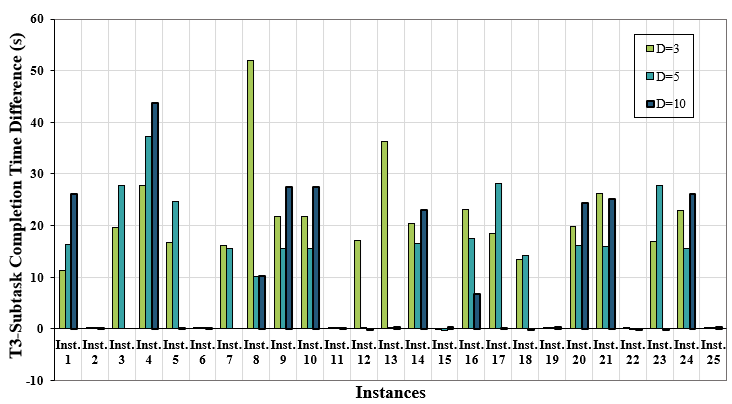
\includegraphics[scale=0.45]{image_15.png}
		\caption{Comparison between TTR (proposed) and TLR. Positive values indicate the superior performance of TTR.}
	\label{test2}
\end{figure}

\subsubsection{Test 3}
In scenarios with multiple collaborative subtasks under limited communication, repeated failures can propagate across temporally dependent tasks and substantially delay mission completion. This test evaluates whether free-market-based reassignment (FMR) can reduce such cascading delays compared with failure-to-tail reassignment (F2TR), where each failed subtask is appended to the end of the local plan and retried later. The comparison is conducted over Inst.~1--Inst.~25 under $D=1.5$\,m, using task completion time as the primary metric. Consider the LTL-specified task
$\varphi_1=\Diamond l^{11}_{1,2}\land \Diamond l^{7}_{1,2}\land \Diamond l^{2}_{1,2}\land \Diamond ((l^{2}_{2,1} \land \lnot l^{9}_{2,2}) \land \Diamond l^{9}_{2,2}).$
Let $\Omega_{\varphi} = \{q_1, q_2, q_3, q_4, q_5\}$, where $q_1 = \{ 1, \{l^2_{2,1}\}\}$, $q_2 = \{2, \{l^9_{2,2}\}\}$, $q_3 = \{3,\{l^2_{1,2}\}\}$, $q_4 = \{4,\{l^{7}_{1,2}\}\}$, and $q_5 = \{5,\{l^{11}_{1,2}\}\}$. Five robots are deployed: ${r_1, r_2, r_3}$ (type 1) and ${r_4, r_5}$ (type 2).

To trigger representative collaborative failures, one type-1 robot is removed before the second (in execution order) type-1 collaborative subtask is completed. This setting is critical because the team has minimal redundancy: a single removal can break the feasibility of the current collaboration and force reallocation. Under F2TR, this often leads to deferral and repeated waiting in downstream subtasks. In contrast, FMR synchronizes failure information in the free market and reallocates with a broader and more up-to-date candidate set, which is expected to reduce repeated failures and shorten recovery latency. From a mechanism perspective, the key difference is whether recovery decisions are made with fragmented local views (F2TR) or with synchronized team-state information (FMR).

%\begin{figure}[thpb]
%	\centering
%	\includegraphics[scale=0.42]{pic/patrol_time.eps}
%	\caption{Task timelines in Test 1 ($D=10$ m). The X-axis is time (seconds), the Y-axis is robots. Wide blocks denote subtasks, narrow colored blocks indicate waiting, and gray lines mean no subtask and not in the free market.}
%	\label{F2TR}
%\end{figure}

\begin{figure}
	\centering
	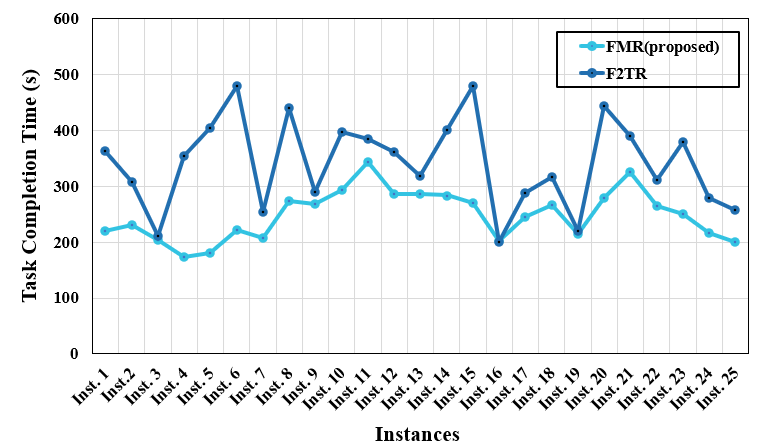
\includegraphics[width=1.0\linewidth]{image_17.png}
	\caption{Comparison between FMR (proposed) and F2TR.}
	\label{F2TR}
\end{figure}


\begin{figure}
	\centering
	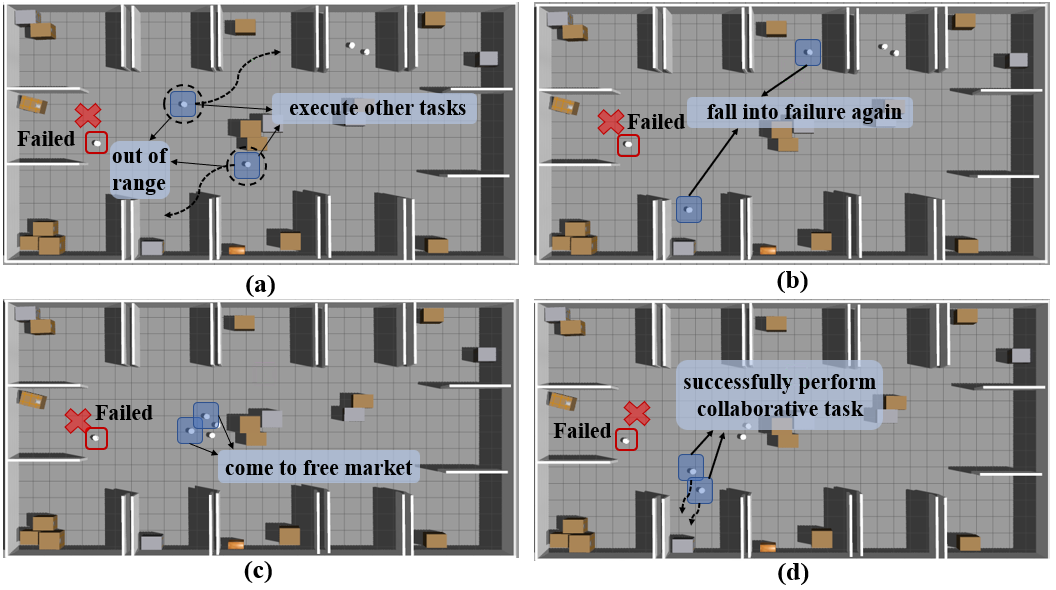
\includegraphics[width=1.0\linewidth]{图3.png}
	\caption{Schematic comparison of collaborative-failure handling processes in F2TR and the proposed method. Subfigures (a) and (b) illustrate the F2TR process, while (c) and (d) illustrate the process of the proposed method.}
	\label{process}
\end{figure}
As shown in Fig.~\ref{F2TR}, FMR generally outperforms F2TR across most instances, indicating that the benefit is systematic rather than case-specific. As shown in Fig.~\ref{process}, the key reason is that, under dense collaborative dependencies and limited communication, a single failure often creates a ``failure--delay--reassignment'' loop: delayed recovery of one subtask postpones its successors, which increases the probability of additional waiting and repeated failures. F2TR tends to amplify this loop because failed subtasks are deferred to the tail and revisited with fragmented local information. In contrast, FMR interrupts the loop by synchronizing failure states in the free market and reallocating from a broader, more up-to-date candidate set, which shortens recovery latency and reduces repeated failure.

The smaller gaps in instances such as Inst.3 and Inst.16 are also informative: when spatial layout and timing naturally permit sufficient information exchange, even local-tail recovery can approach the performance of FMR. This suggests that FMR's main advantage appears in communication-stressed or coordination-dense cases. Overall, the results support that FMR improves not only average completion efficiency but also resilience to chained collaborative-subtask disruptions.
\subsubsection{Test 4}
% At $D=10$ m, with regions $l_1$$\sim$$l_{12}$ arranged as in Fig.~\ref{workspace}, Test 2 introduces both robot addition and robot removal during execution to evaluate online reallocation and collaboration recovery. First, a new type-3 robot $r_{13}$ joins at $t=15$. After entering communication range and synchronizing task-state information, $r_{13}$ is incorporated into the candidate set and assigned to $q_2$, reducing the load on the original team and improving schedule flexibility. Later, robot $r_{10}$ is removed at $t=80$, which causes collaborative subtask $q_1$ to become understaffed. The leader $r_{11}$ then keeps the remaining participants in a waiting state and monitors whether the missing role can be filled locally. When the waiting duration exceeds $T_\mathrm{col}$, $r_{11}$ triggers the timeout-based recovery process and dispatches $r_9$ as a recruiter to obtain a qualified replacement robot. After recruitment succeeds, the team is re-formed and $q_1$ is completed by $r_{11}$, $r_{13}$, and $r_9$ (Fig.~\ref{add}). From a process viewpoint, this case contains a complete "disturbance--response--stabilization" chain: the removal of $r_{10}$ first creates a collaborative-subtask failure risk (insufficient participants for $q_1$), then timeout-triggered recruitment restores the required team size, and finally execution returns to a consistent state. During this transition, shared plan/state information ($\mathcal{P}_k(\tau_n)$ and $\mathcal{S}_k(\tau_n)$) supports real-time conflict detection and mitigation, reducing temporary duplicate or inconsistent assignments that may arise after team-size changes. Therefore, the trajectory in Fig.~\ref{add} reflects not only successful completion, but also the effectiveness of two coupled mechanisms: collaborative-failure recovery and online task-conflict reduction.

At $D=10$\,m, with regions $l_1 \sim l_{12}$ arranged as shown in Fig.~\ref{workspace}, Test~4 evaluates the proposed framework under dynamic changes in team composition by introducing both robot addition and robot removal during task execution. At $t=15$, a new type-3 robot, $r_{13}$, joins the system. After entering the communication range and synchronizing with the team, $r_{13}$ is incorporated into the candidate set and assigned to subtask $q_2$. This online reallocation updates the task assignment according to the new team composition, thereby reducing the burden on the original team and yielding a plan suited to the expanded set of available robots.

Later, at $t=80$, robot $r_{10}$ is removed, leaving collaborative subtask $q_1$ understaffed. In response, the leader robot $r_{11}$ keeps the remaining participants in a waiting state while checking whether the missing role can be filled locally. Once the waiting time exceeds $T_\mathrm{wait}$, $r_{11}$ activates the timeout-based recovery mechanism and dispatches $r_9$ as a recruiter to seek a qualified replacement. After recruitment succeeds, the team is re-formed, and $q_1$ is eventually completed by $r_{11}$, $r_{13}$, and $r_9$, as shown in Fig.~\ref{add}.

From a process perspective, this scenario captures the full evolution from disturbance to response and eventual recovery. Specifically, the removal of $r_{10}$ first introduces the risk of collaborative-subtask failure due to an insufficient number of participants for $q_1$; the timeout-triggered recruitment mechanism then restores the required team size; and finally, task execution returns to a consistent and stable state. Therefore, the trajectory shown in Fig.~\ref{add} demonstrates not only successful task completion, but also the effectiveness of the proposed framework in supporting both collaborative-failure recovery and online task reallocation under dynamic team changes.
\begin{figure}[thpb]
	\centering
	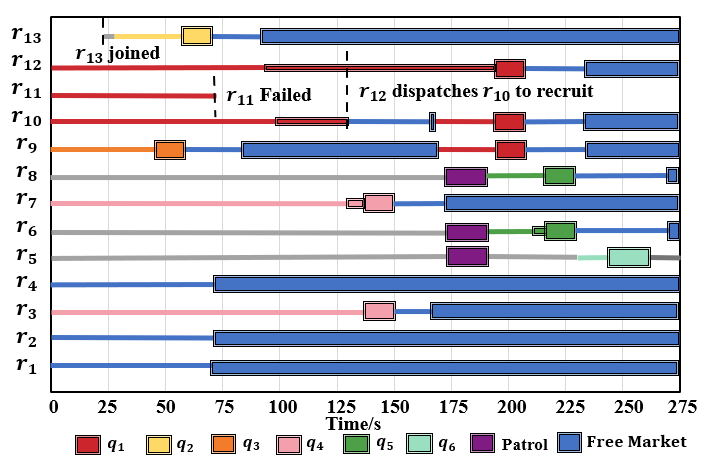
\includegraphics[scale=0.5]{image_26.png}
	\caption{Task timelines in Test 4. Wide blocks denote subtasks, narrow colored blocks indicate waiting. Gray lines mean no subtask and not in the free market, and other colored lines represent traveling toward the target region.}
	\label{add}
\end{figure}


%\begin{table}[h]
%	\caption{SUBTASK COMPLETION TIME UNDER DIFFERENT COMMUNICATION RANGE}
%	\label{tab1}
%	\begin{center}
%		\begin{tabular}{|c|c|c|c|c|}
%			\hline
%			$D$ (m) & 5.0 & 10.0 & 15.0 &  30.0 \\\hline
%			Case 1: with TTR (s) & 140.5& 129.15& 123.65 & 123.45\\
%			\hline
%			Case 2: without TTR (s) & 161.23 & 156.76 & 155.28 & 154.64\\
%			\hline
%			%  Case2 & 219.65 & 214.05 & 176.15 &  162.45& 161.09\\
%			%  \hline
%		\end{tabular}
%	\end{center}
%%	  \smallskip
%%	\small
%%	\textit{Note:} \textsuperscript{*} Proposed method.
%\end{table}

% \subsubsection{Test 3}
% In scenarios with multiple collaborative subtasks under limited communication, repeated failures can propagate across temporally dependent tasks and substantially delay mission completion. This test evaluates whether free-market-based reassignment (FMR) can reduce such cascading delays compared with failure-to-tail reassignment (F2TR), where each failed subtask is appended to the end of the local plan and retried later. The comparison is conducted over Inst.1$\sim$Inst.25 using task completion time as the primary metric.

% Consider the collaboration-intensive task
% \begin{equation}
% \varphi_1=\Diamond l^{11}_{1,2}\land \Diamond l^{7}_{1,2} \land \Diamond l^{2}_{1,2}\land \Diamond (l^{2}_{2,1} \land \Diamond l^{9}_{2,2}).
% \end{equation}
% Let $\Omega_{\varphi} = \{q_1, q_2, q_3, q_4, q_5\}$, where $q_1 = \{ 1, \{l^2_{2,1}\}\}$, $q_2 = \{2, \{l^9_{2,2}\}\}$, $q_3 = \{3,\{l^2_{1,2}\}\}$, $q_4 = \{4,\{l^{7}_{1,2}\}\}$, and $q_5 = \{5,\{l^{11}_{1,2}\}\}$. Five robots are deployed: ${r_1, r_2, r_3}$ (type 1) and ${r_4, r_5}$ (type 2).

% To trigger representative collaborative failures, one type-1 robot is removed before the second (in execution order) type-1 collaborative subtask is completed. This setting is critical because the team has minimal redundancy: a single removal can break feasibility of the current collaboration and force reallocation. Under F2TR, this often leads to deferral and repeated waiting in downstream subtasks. In contrast, FMR synchronizes failure information in the free market and reallocates with a wider, updated candidate set, which is expected to reduce repeated failures and shorten recovery latency. From a mechanism perspective, the key difference is whether recovery decisions are made with fragmented local views (F2TR) or with synchronized team-state information (FMR). Therefore, this experiment is designed not only to compare completion time, but also to verify whether centralized information exchange at the free market improves resilience against chained collaborative-subtask disruptions. We also expect the performance gap to widen as communication becomes sparser, because local-only reassignment becomes more myopic while free-market synchronization preserves global consistency of recovery decisions.

% %\begin{figure}[thpb]
% %	\centering
% %	\includegraphics[scale=0.42]{pic/patrol_time.eps}
% %	\caption{Task timelines in Test 1 ($D=10$ m). The X-axis is time (seconds), the Y-axis is robots. Wide blocks denote subtasks, narrow colored blocks indicate waiting, and gray lines mean no subtask and not in the free market.}
% %	\label{F2TR}
% %\end{figure}

% \begin{figure}
% 	\centering
% 	
\includegraphics[width=0.75\linewidth]{pic/Test4.eps}
% 	\caption{Comparison between FMR (proposed) and F2TR.}
% 	\label{F2TR}
% \end{figure}

% As shown in Fig.~\ref{F2TR}, FMR generally outperforms F2TR across most instances, indicating that the benefit is systematic rather than case-specific. The key reason is that, under dense collaborative dependencies and limited communication, a single failure often creates a "failure--delay--reassignment" loop: delayed recovery of one subtask postpones its successors, which increases the probability of additional waiting and repeated failures. F2TR tends to amplify this loop because failed subtasks are deferred to the tail and revisited with fragmented local information. In contrast, FMR interrupts the loop by synchronizing failure states in the free market and reallocating from a broader, updated candidate set, which shortens recovery latency and reduces repeated failure cycles.

% The smaller gaps in instances such as Inst.3 and Inst.16 are also informative: when spatial layout and timing naturally permit sufficient information exchange, even local-tail recovery can approach the performance of FMR. This suggests that FMR's main advantage appears in communication-stressed or coordination-dense cases, i.e., precisely the operating conditions where robustness is most needed. Overall, the results support that FMR improves not only average completion efficiency but also resilience to chained collaborative-subtask disruptions.

\subsection{Physical Experiment}

Consider the environment depicted in Fig.~\ref{fig:fourgrid}(a), where $l_1$ denotes the sorting area, $l_2$ the storage center, and $l_3$ the monitoring room. Four robots of three distinct types operate with a 2.0-meter communication range. The mission specification $\varphi = \Diamond(l^{1}_{1,1} \land l^{1}_{3,1} \land l^{1}_{2,1}) \land \Diamond l^{2}_{3,1} \land \Diamond l^{3}_{1,1} \land \Diamond l^{2}_{2,1} \land (\neg l^{2}_{2,1} \mathcal{U} \, l^{4}_{1,1}) \land (\neg l^{3}_{1,1} \mathcal{U} \, (l^{1}_{1,1} \land l^{1}_{3,1} \land l^{1}_{2,1}))$ requires one robot of each type (1, 2, and 3) to inspect, classify, and process goods in the sorting area $l_1$; a type-3 robot to inspect the storage area $l_2$; and, upon completion of the sorting tasks, a type-1 robot to report in the monitoring room $l_3$, after which a type-2 robot processes goods in the storage area $l_2$.

Experimental results (Fig.~\ref{fig:fourgrid}) show that the proposed mechanisms are effective in a real communication-limited setting. First, the collaborative operation in $l_1$ is completed before the dependent actions in $l_3$, which is consistent with the temporal-order constraints in $\varphi$ and indicates that prerequisite information is propagated in time to avoid logical blocking. Second, after leaving $l_1$, robot $r_1$ proceeds to $l_3$ while $r_2$ is temporarily outside direct 2.0-meter communication range; nevertheless, team coordination is preserved through free-market-mediated information exchange, so execution does not stall due to link interruption. Third, once the $l_3$-related subtask is confirmed complete, $r_2$ transitions to $l_2$ to execute the subsequent dependent task, showing that task handoff remains consistent even across intermittent connectivity.
Overall, the physical experiment validates three key properties in combination: i) correctness of temporally constrained execution, ii) communication resilience via the free market under range limitations, and iii) continuity of distributed task progression without centralized global replanning.
 

\begin{figure*}[!t]
	\centering
	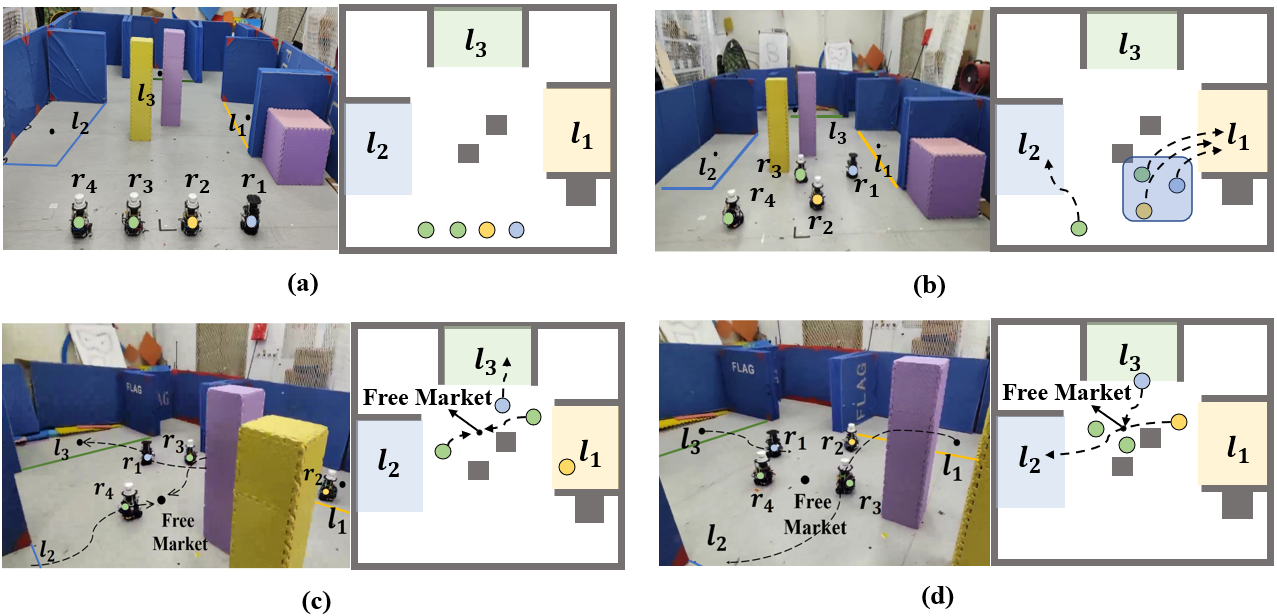
\includegraphics[width=0.8\textwidth]{image_29.png}
	\caption{The dashed lines indicate the robot trajectories. In (a), $l_1$ to $l_3$ represent the areas of interest. There are three kinds of robots: $\{r_1\}$, $\{r_2\}$ and $\{r_3, r_4\}$. In (b)-(d), the robots are executing their subtasks.}
	\label{fig:fourgrid}
\end{figure*}
\section{CONCLUSIONS}

This paper presents a distributed task allocation framework with resilient task coordination for heterogeneous multi-robot systems under temporal logic and communication constraints. Starting from a global sc-LTL specification, the framework derives executable subtasks through automaton pruning and task decomposition, and generates initial plans using CBTA. To sustain task progress under limited communication, the framework incorporates two complementary coordination mechanisms: a patrol mechanism for resolving task blocking through active information gathering, and a coordination mechanism for collaborative subtasks that combines leader-based coordination, timeout-triggered recruitment, and free-market-based reassignment. Theoretical analysis establishes task-completion guarantees under the assumptions of this paper. Simulations on 25 benchmark instances and a physical experiment demonstrate that the proposed framework improves the robustness of distributed task coordination under incomplete and delayed team-state information.
% \begin{equation}
% \label{deqn_ex1a}
% x = \sum_{i=0}^{n} 2{i} Q.
% \end{equation}


% \section{Some Common Elements}
% \subsection{Sections and Subsections}
% Enumeration of section headings is desirable, but not required. When numbered, please be consistent throughout the article, that is, all headings and all levels of section headings in the article should be enumerated. Primary headings are designated with Roman numerals, secondary with capital letters, tertiary with Arabic numbers; and quaternary with lowercase letters. Reference and Acknowledgment headings are unlike all other section headings in text. They are never enumerated. They are simply primary headings without labels, regardless of whether the other headings in the article are enumerated.

% \subsection{Citations to the Bibliography}
% The coding for the citations is made with the \LaTeX\ $\backslash${\tt{cite}} command.
% This will display as: see \cite{ref1}.

% For multiple citations code as follows: {\tt{$\backslash$cite\{ref1,ref2,ref3\}}}
%  which will produce \cite{ref1,ref2,ref3}. For reference ranges that are not consecutive code as {\tt{$\backslash$cite\{ref1,ref2,ref3,ref9\}}} which will produce  \cite{ref1,ref2,ref3,ref9}

% \subsection{Lists}
% In this section, we will consider three types of lists: simple unnumbered, numbered, and bulleted. There have been many options added to IEEEtran to enhance the creation of lists. If your lists are more complex than those shown below, please refer to the original ``IEEEtran\_HOWTO.pdf'' for additional options.\\

% \subsubsection*{\bf A plain  unnumbered list}
% \begin{list}{}{}
% \item{bare\_jrnl.tex}
% \item{bare\_conf.tex}
% \item{bare\_jrnl\_compsoc.tex}
% \item{bare\_conf\_compsoc.tex}
% \item{bare\_jrnl\_comsoc.tex}
% \end{list}

% \subsubsection*{\bf A simple numbered list}
% \begin{enumerate}
% \item{bare\_jrnl.tex}
% \item{bare\_conf.tex}
% \item{bare\_jrnl\_compsoc.tex}
% \item{bare\_conf\_compsoc.tex}
% \item{bare\_jrnl\_comsoc.tex}
% \end{enumerate}

% \subsubsection*{\bf A simple bulleted list}
% \begin{itemize}
% \item{bare\_jrnl.tex}
% \item{bare\_conf.tex}
% \item{bare\_jrnl\_compsoc.tex}
% \item{bare\_conf\_compsoc.tex}
% \item{bare\_jrnl\_comsoc.tex}
% \end{itemize}





% \subsection{Figures}
% Fig. 1 is an example of a floating figure using the graphicx package.
%  Note that $\backslash${\tt{label}} must occur AFTER (or within) $\backslash${\tt{caption}}.
%  For figures, $\backslash${\tt{caption}} should occur after the $\backslash${\tt{includegraphics}}.

% \begin{figure}[!t]
% \centering
% 
\includegraphics[width=2.5in]{fig1}
% \caption{Simulation results for the network.}
% \label{fig_1}
% \end{figure}

% Fig. 2(a) and 2(b) is an example of a double column floating figure using two subfigures.
%  (The subfig.sty package must be loaded for this to work.)
%  The subfigure $\backslash${\tt{label}} commands are set within each subfloat command,
%  and the $\backslash${\tt{label}} for the overall figure must come after $\backslash${\tt{caption}}.
%  $\backslash${\tt{hfil}} is used as a separator to get equal spacing.
%  The combined width of all the parts of the figure should do not exceed the text width or a line break will occur.
% %
% \begin{figure*}[!t]
% \centering
% \subfloat[]{
\includegraphics[width=2.5in]{fig1}%
% \label{fig_first_case}}
% \hfil
% \subfloat[]{
\includegraphics[width=2.5in]{fig1}%
% \label{fig_second_case}}
% \caption{Dae. Ad quatur autat ut porepel itemoles dolor autem fuga. Bus quia con nessunti as remo di quatus non perum que nimus. (a) Case I. (b) Case II.}
% \label{fig_sim}
% \end{figure*}

% Note that often IEEE papers with multi-part figures do not place the labels within the image itself (using the optional argument to $\backslash${\tt{subfloat}}[]), but instead will
%  reference/describe all of them (a), (b), etc., within the main caption.
%  Be aware that for subfig.sty to generate the (a), (b), etc., subfigure
%  labels, the optional argument to $\backslash${\tt{subfloat}} must be present. If a
%  subcaption is not desired, leave its contents blank,
%  e.g.,$\backslash${\tt{subfloat}}[].




% \section{Tables}
% Note that, for IEEE-style tables, the
%  $\backslash${\tt{caption}} command should come BEFORE the table. Table captions use title case. Articles (a, an, the), coordinating conjunctions (and, but, for, or, nor), and most short prepositions are lowercase unless they are the first or last word. Table text will default to $\backslash${\tt{footnotesize}} as
%  the IEEE normally uses this smaller font for tables.
%  The $\backslash${\tt{label}} must come after $\backslash${\tt{caption}} as always.

% \begin{table}[!t]
% \caption{An Example of a Table\label{tab:table1}}
% \centering
% \begin{tabular}{|c||c|}
% \hline
% One & Two\\
% \hline
% Three & Four\\
% \hline
% \end{tabular}
% \end{table}

% \section{Algorithms}
% Algorithms should be numbered and include a short title. They are set off from the text with rules above and below the title and after the last line.

% \begin{algorithm}[H]
% \caption{Weighted Tanimoto ELM.}\label{alg:alg1}
% \begin{algorithmic}
% \STATE
% \STATE {\textsc{TRAIN}}$(\mathbf{X} \mathbf{T})$
% \STATE \hspace{0.5cm}$ \textbf{select randomly } W \subset \mathbf{X}  $
% \STATE \hspace{0.5cm}$ N_\mathbf{t} \gets | \{ i : \mathbf{t}_i = \mathbf{t} \} | $ \textbf{ for } $ \mathbf{t}= -1,+1 $
% \STATE \hspace{0.5cm}$ B_i \gets \sqrt{ \textsc{max}(N_{-1},N_{+1}) / N_{\mathbf{t}_i} } $ \textbf{ for } $ i = 1,...,N $
% \STATE \hspace{0.5cm}$ \hat{\mathbf{H}} \gets  B \cdot (\mathbf{X}^T\textbf{W})/( \mathbb{1}\mathbf{X} + \mathbb{1}\textbf{W} - \mathbf{X}^T\textbf{W} ) $
% \STATE \hspace{0.5cm}$ \beta \gets \left ( I/C + \hat{\mathbf{H}}^T\hat{\mathbf{H}} \right )^{-1}(\hat{\mathbf{H}}^T B\cdot \mathbf{T})  $
% \STATE \hspace{0.5cm}\textbf{return}  $\textbf{W},  \beta $
% \STATE
% \STATE {\textsc{PREDICT}}$(\mathbf{X} )$
% \STATE \hspace{0.5cm}$ \mathbf{H} \gets  (\mathbf{X}^T\textbf{W} )/( \mathbb{1}\mathbf{X}  + \mathbb{1}\textbf{W}- \mathbf{X}^T\textbf{W}  ) $
% \STATE \hspace{0.5cm}\textbf{return}  $\textsc{sign}( \mathbf{H} \beta )$
% \end{algorithmic}
% \label{alg1}
% \end{algorithm}

% Que sunt eum lam eos si dic to estist, culluptium quid qui nestrum nobis reiumquiatur minimus minctem. Ro moluptat fuga. Itatquiam ut laborpo rersped exceres vollandi repudaerem. Ulparci sunt, qui doluptaquis sumquia ndestiu sapient iorepella sunti veribus. Ro moluptat fuga. Itatquiam ut laborpo rersped exceres vollandi repudaerem.
% \section{Mathematical Typography \\ and Why It Matters}

% Typographical conventions for mathematical formulas have been developed to {\bf provide uniformity and clarity of presentation across mathematical texts}. This enables the readers of those texts to both understand the author's ideas and to grasp new concepts quickly. While software such as \LaTeX \ and MathType\textsuperscript{\textregistered} can produce aesthetically pleasing math when used properly, it is also very easy to misuse the software, potentially resulting in incorrect math display.

% IEEE aims to provide authors with the proper guidance on mathematical typesetting style and assist them in writing the best possible article. As such, IEEE has assembled a set of examples of good and bad mathematical typesetting \cite{ref1,ref2,ref3,ref4,ref5}.

% Further examples can be found at \url{http://journals.ieeeauthorcenter.ieee.org/wp-content/uploads/sites/7/IEEE-Math-Typesetting-Guide-for-LaTeX-Users.pdf}

% \subsection{Display Equations}
% The simple display equation example shown below uses the ``equation'' environment. To number the equations, use the $\backslash${\tt{label}} macro to create an identifier for the equation. LaTeX will automatically number the equation for you.
% \begin{equation}
% \label{deqn_ex1}
% x = \sum_{i=0}^{n} 2{i} Q.
% \end{equation}

% \noindent is coded as follows:
% \begin{verbatim}
% \begin{equation}
% \label{deqn_ex1}
% x = \sum_{i=0}^{n} 2{i} Q.
% \end{equation}
% \end{verbatim}

% To reference this equation in the text use the $\backslash${\tt{ref}} macro.
% Please see (\ref{deqn_ex1})\\
% \noindent is coded as follows:
% \begin{verbatim}
% Please see (\ref{deqn_ex1})\end{verbatim}

% \subsection{Equation Numbering}
% {\bf{Consecutive Numbering:}} Equations within an article are numbered consecutively from the beginning of the
% article to the end, i.e., (1), (2), (3), (4), (5), etc. Do not use roman numerals or section numbers for equation numbering.

% \noindent {\bf{Appendix Equations:}} The continuation of consecutively numbered equations is best in the Appendix, but numbering
%  as (A1), (A2), etc., is permissible.\\

% \noindent {\bf{Hyphens and Periods}}: Hyphens and periods should not be used in equation numbers, i.e., use (1a) rather than
% (1-a) and (2a) rather than (2.a) for subequations. This should be consistent throughout the article.

% \subsection{Multi-Line Equations and Alignment}
% Here we show several examples of multi-line equations and proper alignments.

% \noindent {\bf{A single equation that must break over multiple lines due to length with no specific alignment.}}
% \begin{multline}
% \text{The first line of this example}\\
% \text{The second line of this example}\\
% \text{The third line of this example}
% \end{multline}

% \noindent is coded as:
% \begin{verbatim}
% \begin{multline}
% \text{The first line of this example}\\
% \text{The second line of this example}\\
% \text{The third line of this example}
% \end{multline}
% \end{verbatim}

% \noindent {\bf{A single equation with multiple lines aligned at the = signs}}
% \begin{align}
% a &= c+d \\
% b &= e+f
% \end{align}
% \noindent is coded as:
% \begin{verbatim}
% \begin{align}
% a &= c+d \\
% b &= e+f
% \end{align}
% \end{verbatim}

% The {\tt{align}} environment can align on multiple  points as shown in the following example:
% \begin{align}
% x &= y & X & =Y & a &=bc\\
% x' &= y' & X' &=Y' &a' &=bz
% \end{align}
% \noindent is coded as:
% \begin{verbatim}
% \begin{align}
% x &= y & X & =Y & a &=bc\\
% x' &= y' & X' &=Y' &a' &=bz
% \end{align}
% \end{verbatim}





% \subsection{Subnumbering}
% The amsmath package provides a {\tt{subequations}} environment to facilitate subnumbering. An example:

% \begin{subequations}\label{eq:2}
% \begin{align}
% f&=g \label{eq:2A}\\
% f' &=g' \label{eq:2B}\\
% \mathcal{L}f &= \mathcal{L}g \label{eq:2c}
% \end{align}
% \end{subequations}

% \noindent is coded as:
% \begin{verbatim}
% \begin{subequations}\label{eq:2}
% \begin{align}
% f&=g \label{eq:2A}\\
% f' &=g' \label{eq:2B}\\
% \mathcal{L}f &= \mathcal{L}g \label{eq:2c}
% \end{align}
% \end{subequations}

% \end{verbatim}

% \subsection{Matrices}
% There are several useful matrix environments that can save you some keystrokes. See the example coding below and the output.

% \noindent {\bf{A simple matrix:}}
% \begin{equation}
% \begin{matrix}  0 &  1 \\
% 1 &  0 \end{matrix}
% \end{equation}
% is coded as:
% \begin{verbatim}
% \begin{equation}
% \begin{matrix}  0 &  1 \\
% 1 &  0 \end{matrix}
% \end{equation}
% \end{verbatim}

% \noindent {\bf{A matrix with parenthesis}}
% \begin{equation}
% \begin{pmatrix} 0 & -i \\
%  i &  0 \end{pmatrix}
% \end{equation}
% is coded as:
% \begin{verbatim}
% \begin{equation}
% \begin{pmatrix} 0 & -i \\
%  i &  0 \end{pmatrix}
% \end{equation}
% \end{verbatim}

% \noindent {\bf{A matrix with square brackets}}
% \begin{equation}
% \begin{bmatrix} 0 & -1 \\
% 1 &  0 \end{bmatrix}
% \end{equation}
% is coded as:
% \begin{verbatim}
% \begin{equation}
% \begin{bmatrix} 0 & -1 \\
% 1 &  0 \end{bmatrix}
% \end{equation}
% \end{verbatim}

% \noindent {\bf{A matrix with curly braces}}
% \begin{equation}
% \begin{Bmatrix} 1 &  0 \\
% 0 & -1 \end{Bmatrix}
% \end{equation}
% is coded as:
% \begin{verbatim}
% \begin{equation}
% \begin{Bmatrix} 1 &  0 \\
% 0 & -1 \end{Bmatrix}
% \end{equation}\end{verbatim}

% \noindent {\bf{A matrix with single verticals}}
% \begin{equation}
% \begin{vmatrix} a &  b \\
% c &  d \end{vmatrix}
% \end{equation}
% is coded as:
% \begin{verbatim}
% \begin{equation}
% \begin{vmatrix} a &  b \\
% c &  d \end{vmatrix}
% \end{equation}\end{verbatim}

% \noindent {\bf{A matrix with double verticals}}
% \begin{equation}
% \begin{Vmatrix} i &  0 \\
% 0 & -i \end{Vmatrix}
% \end{equation}
% is coded as:
% \begin{verbatim}
% \begin{equation}
% \begin{Vmatrix} i &  0 \\
% 0 & -i \end{Vmatrix}
% \end{equation}\end{verbatim}

% \subsection{Arrays}
% The {\tt{array}} environment allows you some options for matrix-like equations. You will have to manually key the fences, but there are other options for alignment of the columns and for setting horizontal and vertical rules. The argument to {\tt{array}} controls alignment and placement of vertical rules.

% A simple array
% \begin{equation}
% \left(
% \begin{array}{cccc}
% a+b+c & uv & x-y & 27\\
% a+b & u+v & z & 134
% \end{array}\right)
% \end{equation}
% is coded as:
% \begin{verbatim}
% \begin{equation}
% \left(
% \begin{array}{cccc}
% a+b+c & uv & x-y & 27\\
% a+b & u+v & z & 134
% \end{array} \right)
% \end{equation}
% \end{verbatim}

% A slight variation on this to better align the numbers in the last column
% \begin{equation}
% \left(
% \begin{array}{cccr}
% a+b+c & uv & x-y & 27\\
% a+b & u+v & z & 134
% \end{array}\right)
% \end{equation}
% is coded as:
% \begin{verbatim}
% \begin{equation}
% \left(
% \begin{array}{cccr}
% a+b+c & uv & x-y & 27\\
% a+b & u+v & z & 134
% \end{array} \right)
% \end{equation}
% \end{verbatim}

% An array with vertical and horizontal rules
% \begin{equation}
% \left( \begin{array}{c|c|c|r}
% a+b+c & uv & x-y & 27\\ \hline
% a+b & u+v & z & 134
% \end{array}\right)
% \end{equation}
% is coded as:
% \begin{verbatim}
% \begin{equation}
% \left(
% \begin{array}{c|c|c|r}
% a+b+c & uv & x-y & 27\\
% a+b & u+v & z & 134
% \end{array} \right)
% \end{equation}
% \end{verbatim}
% Note the argument now has the pipe "$\vert$" included to indicate the placement of the vertical rules.


% \subsection{Cases Structures}
% Many times cases can be miscoded using the wrong environment, i.e., {\tt{array}}. Using the {\tt{cases}} environment will save keystrokes (from not having to type the $\backslash${\tt{left}}$\backslash${\tt{lbrace}}) and automatically provide the correct column alignment.
% \begin{equation*}
% {z_m(t)} = \begin{cases}
% 1,&{\text{if}}\ {\beta }_m(t) \\
% {0,}&{\text{otherwise.}}
% \end{cases}
% \end{equation*}
% \noindent is coded as follows:
% \begin{verbatim}
% \begin{equation*}
% {z_m(t)} =
% \begin{cases}
% 1,&{\text{if}}\ {\beta }_m(t),\\
% {0,}&{\text{otherwise.}}
% \end{cases}
% \end{equation*}
% \end{verbatim}
% \noindent Note that the ``\&'' is used to mark the tabular alignment. This is important to get  proper column alignment. Do not use $\backslash${\tt{quad}} or other fixed spaces to try and align the columns. Also, note the use of the $\backslash${\tt{text}} macro for text elements such as ``if'' and ``otherwise.''

% \subsection{Function Formatting in Equations}
% Often, there is an easy way to properly format most common functions. Use of the $\backslash$ in front of the function name will in most cases, provide the correct formatting. When this does not work, the following example provides a solution using the $\backslash${\tt{text}} macro:

% \begin{equation*}
%   d_{R}^{KM} = \underset {d_{l}^{KM}} {\text{arg min}} \{ d_{1}^{KM},\ldots,d_{6}^{KM}\}.
% \end{equation*}

% \noindent is coded as follows:
% \begin{verbatim}
% \begin{equation*}
%  d_{R}^{KM} = \underset {d_{l}^{KM}}
%  {\text{arg min}} \{ d_{1}^{KM},
%  \ldots,d_{6}^{KM}\}.
% \end{equation*}
% \end{verbatim}

% \subsection{ Text Acronyms Inside Equations}
% This example shows where the acronym ``MSE" is coded using $\backslash${\tt{text\{\}}} to match how it appears in the text.

% \begin{equation*}
%  \text{MSE} = \frac {1}{n}\sum _{i=1}^{n}(Y_{i} - \hat {Y_{i}})^{2}
% \end{equation*}

% \begin{verbatim}
% \begin{equation*}
%  \text{MSE} = \frac {1}{n}\sum _{i=1}^{n}
% (Y_{i} - \hat {Y_{i}})^{2}
% \end{equation*}
% \end{verbatim}

% \section{Conclusion}
% The conclusion goes here.


% \section*{Acknowledgments}
% This should be a simple paragraph before the References to thank those individuals and institutions who have supported your work on this article.



% {\appendix[Proof of the Zonklar Equations]
% Use $\backslash${\tt{appendix}} if you have a single appendix:
% Do not use $\backslash${\tt{section}} anymore after $\backslash${\tt{appendix}}, only $\backslash${\tt{section*}}.
% If you have multiple appendixes use $\backslash${\tt{appendices}} then use $\backslash${\tt{section}} to start each appendix.
% You must declare a $\backslash${\tt{section}} before using any $\backslash${\tt{subsection}} or using $\backslash${\tt{label}} ($\backslash${\tt{appendices}} by itself
%  starts a section numbered zero.)}



% %{\appendices
% %\section*{Proof of the First Zonklar Equation}
% %Appendix one text goes here.
% % You can choose not to have a title for an appendix if you want by leaving the argument blank
% %\section*{Proof of the Second Zonklar Equation}
% %Appendix two text goes here.}



% % \section{References Section}
% % You can use a bibliography generated by BibTeX as a .bbl file.
% %  BibTeX documentation can be easily obtained at:
% %  http://mirror.ctan.org/biblio/bibtex/contrib/doc/
% %  The IEEEtran BibTeX style support page is:
% %  http://www.michaelshell.org/tex/ieeetran/bibtex/

%  % argument is your BibTeX string definitions and bibliography database(s)
\bibliographystyle{IEEEtran}
\bibliography{reference}

%
% \section{Simple References}
% You can manually copy in the resultant .bbl file and set second argument of $\backslash${\tt{begin}} to the number of references
%  (used to reserve space for the reference number labels box).

% \begin{thebibliography}{1}
% \bibliographystyle{IEEEtran}

% \bibitem{ref1}
% {\it{Mathematics Into Type}}. American Mathematical Society. [Online]. Available: https://www.ams.org/arc/styleguide/mit-2.pdf

% \bibitem{ref2}
% T. W. Chaundy, P. R. Barrett and C. Batey, {\it{The Printing of Mathematics}}. London, U.K., Oxford Univ. Press, 1954.

% \bibitem{ref3}
% F. Mittelbach and M. Goossens, {\it{The \LaTeX Companion}}, 2nd ed. Boston, MA, USA: Pearson, 2004.

% \bibitem{ref4}
% G. Gr\"atzer, {\it{More Math Into LaTeX}}, New York, NY, USA: Springer, 2007.

% \bibitem{ref5}M. Letourneau and J. W. Sharp, {\it{AMS-StyleGuide-online.pdf,}} American Mathematical Society, Providence, RI, USA, [Online]. Available: http://www.ams.org/arc/styleguide/index.html

% \bibitem{ref6}
% H. Sira-Ramirez, ``On the sliding mode control of nonlinear systems,'' \textit{Syst. Control Lett.}, vol. 19, pp. 303--312, 1992.

% \bibitem{ref7}
% A. Levant, ``Exact differentiation of signals with unbounded higher derivatives,''  in \textit{Proc. 45th IEEE Conf. Decis.
% Control}, San Diego, CA, USA, 2006, pp. 5585--5590. DOI: 10.1109/CDC.2006.377165.

% \bibitem{ref8}
% M. Fliess, C. Join, and H. Sira-Ramirez, ``Non-linear estimation is easy,'' \textit{Int. J. Model., Ident. Control}, vol. 4, no. 1, pp. 12--27, 2008.

% \bibitem{ref9}
% R. Ortega, A. Astolfi, G. Bastin, and H. Rodriguez, ``Stabilization of food-chain systems using a port-controlled Hamiltonian description,'' in \textit{Proc. Amer. Control Conf.}, Chicago, IL, USA,
% 2000, pp. 2245--2249.

% \end{thebibliography}


% \newpage

% \section{Biography Section}
% If you have an EPS/PDF photo (graphicx package needed), extra braces are
%  needed around the contents of the optional argument to biography to prevent
%  the LaTeX parser from getting confused when it sees the complicated
%  $\backslash${\tt{includegraphics}} command within an optional argument. (You can create
%  your own custom macro containing the $\backslash${\tt{includegraphics}} command to make things
%  simpler here.)

% \vspace{11pt}

% \bf{If you include a photo:}\vspace{-33pt}
% \begin{IEEEbiography}[{
\includegraphics[width=1in,height=1.25in,clip,keepaspectratio]{fig1}}]{Michael Shell}
% Use $\backslash${\tt{begin\{IEEEbiography\}}} and then for the 1st argument use $\backslash${\tt{includegraphics}} to declare and link the author photo.
% Use the author name as the 3rd argument followed by the biography text.
% \end{IEEEbiography}

% \vspace{11pt}

% \bf{If you will not include a photo:}\vspace{-33pt}
% \begin{IEEEbiographynophoto}{John Doe}
% Use $\backslash${\tt{begin\{IEEEbiographynophoto\}}} and the author name as the argument followed by the biography text.
% \end{IEEEbiographynophoto}




% \vfill

\end{document}
